\documentclass{beamer}
\usepackage{default}
\usepackage{amsmath}
\usepackage{graphicx}
\usepackage{adjustbox}  % Allows for fitting tables into slide
\usepackage{hyperref}
\usepackage{threeparttable}
\usepackage{caption}
%\usepackage{subcaption}
\usepackage{natbib}
\usepackage{adjustbox}
\usepackage{subcaption}
\usepackage{verbatim}

%\usetheme{AnnArbor}
%\usetheme{Antibes}
%\usetheme{Bergen}
%\usetheme{Berkeley}
%\usetheme{Berlin}
\usetheme{Boadilla}
%\usetheme{boxes}
%\usetheme{CambridgeUS}
%\usetheme{Copenhagen}
%\usetheme{Darmstadt}
%\usetheme{default}
%\usetheme{Frankfurt}
%\usetheme{Goettingen}
%\usetheme{Hannover}
%\usetheme{Ilmenau}
%\usetheme{JuanLesPins}
%\usetheme{Luebeck}
%\usetheme{Madrid}
%\usetheme{Malmoe}
%\usetheme{Marburg}
%\usetheme{Montpellier}
%\usetheme{PaloAlto}
%\usetheme{Pittsburgh}
%\usetheme{Rochester}
%\usetheme{Singapore}
%\usetheme{Szeged}
%\usetheme{Warsaw}


\title{Rigidity of Expectations: Additional Evidence from Density Forecasts of Professionals and Households}

% A subtitle is optional and this may be deleted

\author{Tao Wang \\ Johns Hopkins University}
% - Give the names in the same order as the appear in the paper.
% - Use the \inst{?} command only if the authors have different
%   affiliation.

\date{\today}
% - Either use conference name or its abbreviation.
% - Not really informative to the audience, more for people (including
%   yourself) who are reading the slides online

% This is only inserted into the PDF information catalog. Can be left
% out. 

% If you have a file called "university-logo-filename.xxx", where xxx
% is a graphic format that can be processed by latex or pdflatex,
% resp., then you can add a logo as follows:

% \pgfdeclareimage[height=0.5cm]{university-logo}{university-logo-filename}
% \logo{\pgfuseimage{university-logo}}

% Delete this, if you do not want the table of contents to pop up at
% the beginning of each subsection:
\AtBeginSubsection[]
{
	\begin{frame}<beamer>{Outline}
	\tableofcontents[currentsection]
\end{frame}
}

\begin{document}
	

\begin{frame}
	\titlepage
\end{frame}
\begin{frame}{Outline}
	\tableofcontents
	% You might wish to add the option [pausesections]
\end{frame}


\section{Motivation}

\begin{frame}{Motivation}
	\begin{itemize}
		\item there are various theories on  ``irrational expectation''
		\item different theories can be tested using survey data  in a comparable manner  (\citet{coibion2012can})
		\item a good theory needs to be (relatively) consistent in predictions across different moments
		\item higher moments, i.e. uncertainty, brings about one more restriction
		\item survey also contains information about data generating process itself
	\end{itemize}
\end{frame}


\begin{frame}{What this paper does}
	\begin{enumerate}
		\item time series and cross-sectional pattern of \textcolor{blue}{uncertainty} from \textbf{density} forecasts of the inflation 
		\item additional reduced-form tests of the full-information rationality null using the uncertainty 
		\item extend \citet{coibion2012can} in two ways 
		\begin{itemize}
		\item cross-moment estimation for each one of the particular theories on expectation 
		\item allowing for stochastic volatility of inflation process 
		\end{itemize}
	\end{enumerate}
\end{frame}


\begin{frame}{Literature}
\begin{itemize}
	\item empirical tests on expectation formation
	\begin{itemize}
		\item \citet{mankiw2003disagreement}, \citet{carroll2003macroeconomic}, \citet{branch2004theory}, \citet{malmendier2015learning}, \citet{das2017socioeconomic}, \citet{coibion2012can}, \citet{fuhrer2018intrinsic} 
	\end{itemize}
    \item density and probabilistic questions in expectation surveys
    \begin{itemize}
    	\item  \citet{manski2004measuring}, \citet{delavande2011measuring}, \citet{manski2018survey} 
    	\item  \citet{bertrand2001people},  \citet{van2008rethinking},  \citet{delavande2014probabilistic}
    \end{itemize}
    \item different measures of uncertainty
    \begin{itemize}
    	\item \citet{bachmann2013uncertainty},  \citet{jurado2015measuring}, \citet{binder2017measuring},  \citet{bloom2009impact}
    \end{itemize}
\end{itemize}
\end{frame}

\begin{frame}{A generic framework}
	
	h-period ahead density forecast by agent $i$ at time $t$ based on information set $I_{i,t}$
	
	\begin{eqnarray*}
		f_{i,t+h|t} \equiv f_{i,t}(y_{t+h}|I_{i,t})
	\end{eqnarray*}
	
	\begin{itemize}
		\item theories of expectation differ in $I_{i,t}$ 
		\begin{itemize}
			\item rational expectation (FIRE): $I_{i,t} = y_{i,t}$
			\item sticky expectation (SE):  $I_{i,t} = y_{t-\tau}$, $\tau$ being the most recent update date
			\item noisy information (NI): $I_{i,t} = s_{i,t}(y_t)$, where $s_{i,t}$ is a vector of noisy signal(s)
		\end{itemize}
		\item the process of variable determines the mapping from $I_{i,t}$ to $f_{i,t+h|t}$
	\end{itemize}
\end{frame}


\begin{frame}{Definition and notation}
	\begin{table}[ht]
		\centering
		\label{MomSum}
		\begin{tabular}{ll}
			
			\hline 
			Individual moments                                  & Population moments                             \\
			\hline 
			Mean forecast: $y_{i,t+h|t}$                   & Average forecast: $\bar y_{t+h|t}$                   \\
			Forecast error: $FE_{i,t+h|t}$ & Average forecast error: $\overline{FE}_{t+h|t}$ \\
			Uncertainty: $Var_{i,t+h|t}$         & \textbf{Average uncertainty}:  $\overline{Var}_{t+h|t}$ \\
			& Disagreement:  $\overline{Disg}_{t+h|t}$       \\
			\hline 
		\end{tabular}
	\end{table}
	
\end{frame}


\begin{frame}{Data}
	\begin{table}[]
		\resizebox{\textwidth}{!}{	\begin{tabular}{lll}
				
				\hline 
				& SCE & SPF        \\
				\hline 
				Time period                                    & 2013M6-2018M6                            & 2007Q1-2018Q4             \\
				Frequency                                      & Monthly                                 & Quarterly                \\
				Sample Size                                    & 1,300                                   & 30-50                    \\
				Aggregate Var in Density                       & \textcolor{blue}{1-yr-ahead inflation}          & \textcolor{blue}{1-yr and 3-yr core CPI and core PCE}         \\
				Pannel Structure                               & stay up to 12 months                    & average stay for 5 years \\
				Demographic Info                        & Education, Income, Age        & Industry    \\
				\hline 
		\end{tabular}}
	\end{table}
\begin{itemize}
	\item density estimation following (\citet{engelberg2009comparing})
	\item exclude top and bottom 5\% values for forecast errors and uncertainty
\end{itemize}
\end{frame}


\begin{frame}{Basic patterns: uncertainty and realized inflation}
	\begin{figure}
		\centering
		\label{InfVar}
		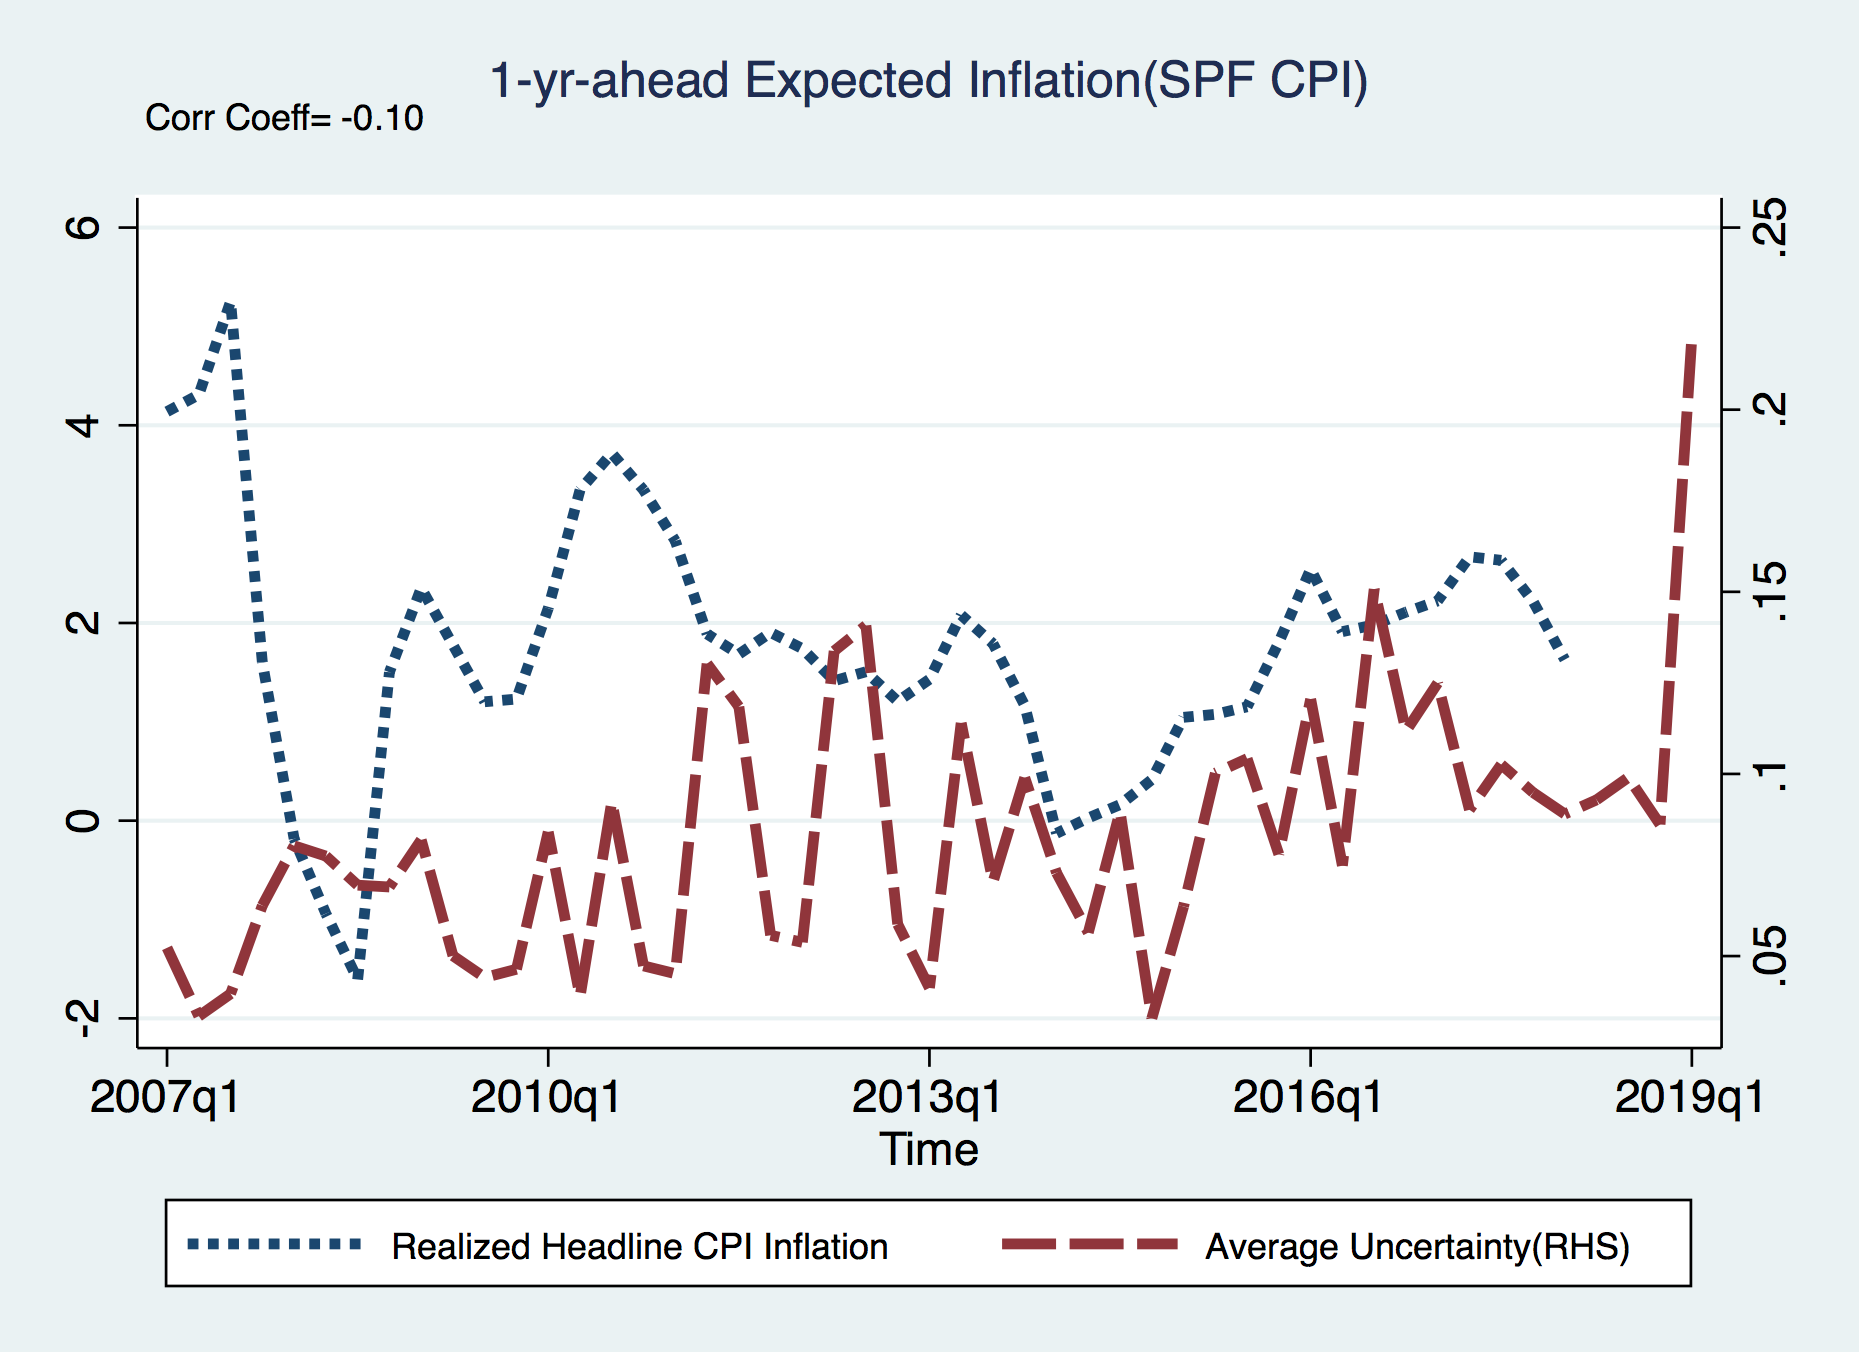
\includegraphics[width=0.3\textwidth]{figuresDraft/Inf1yf_CPIAU_varSPFCPIQ.png}
		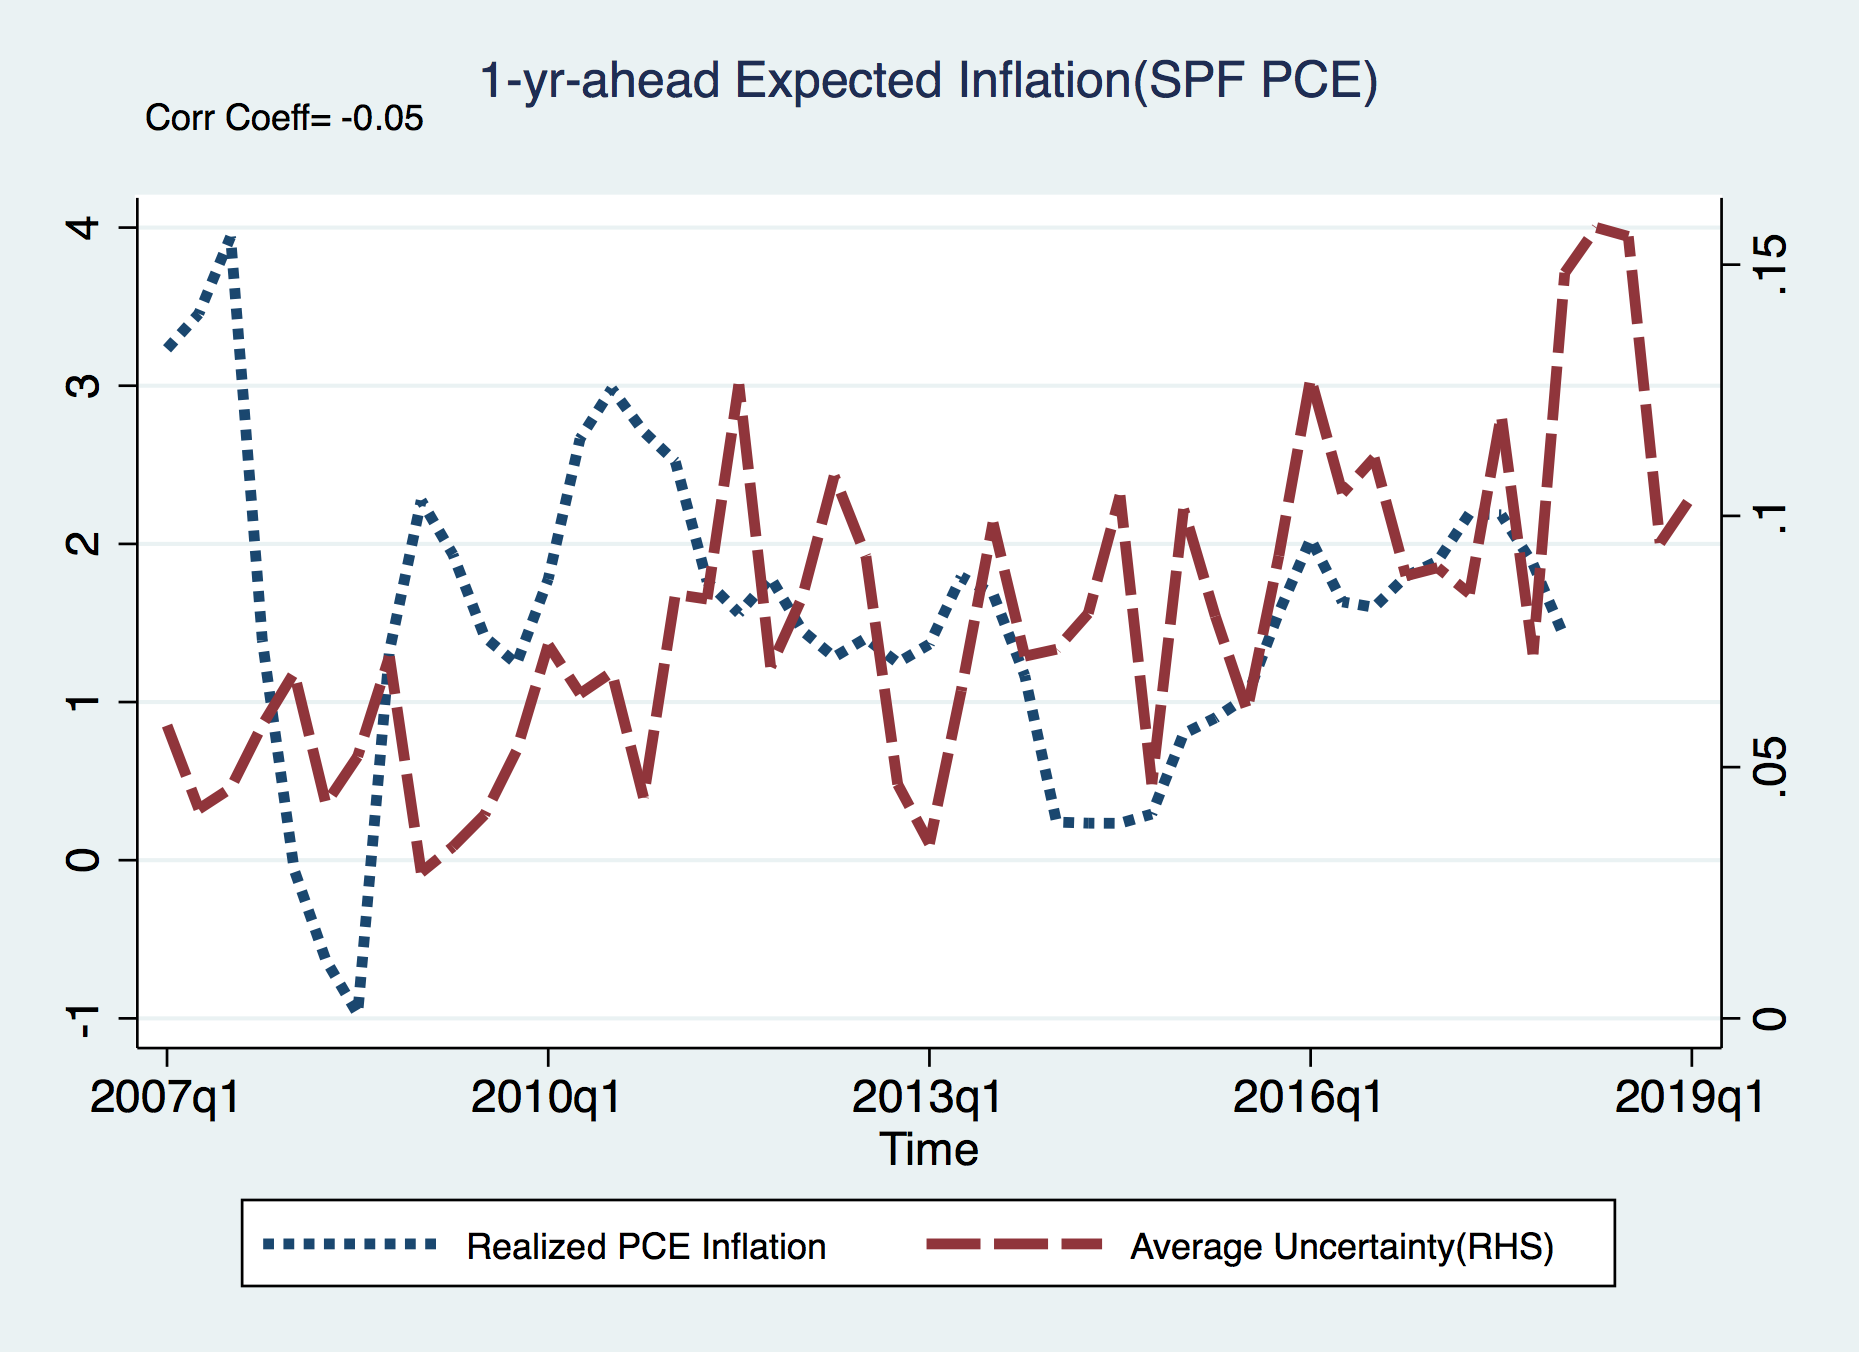
\includegraphics[width=0.3\textwidth]{figuresDraft/Inf1yf_PCE_varSPFPCEQ.png}
		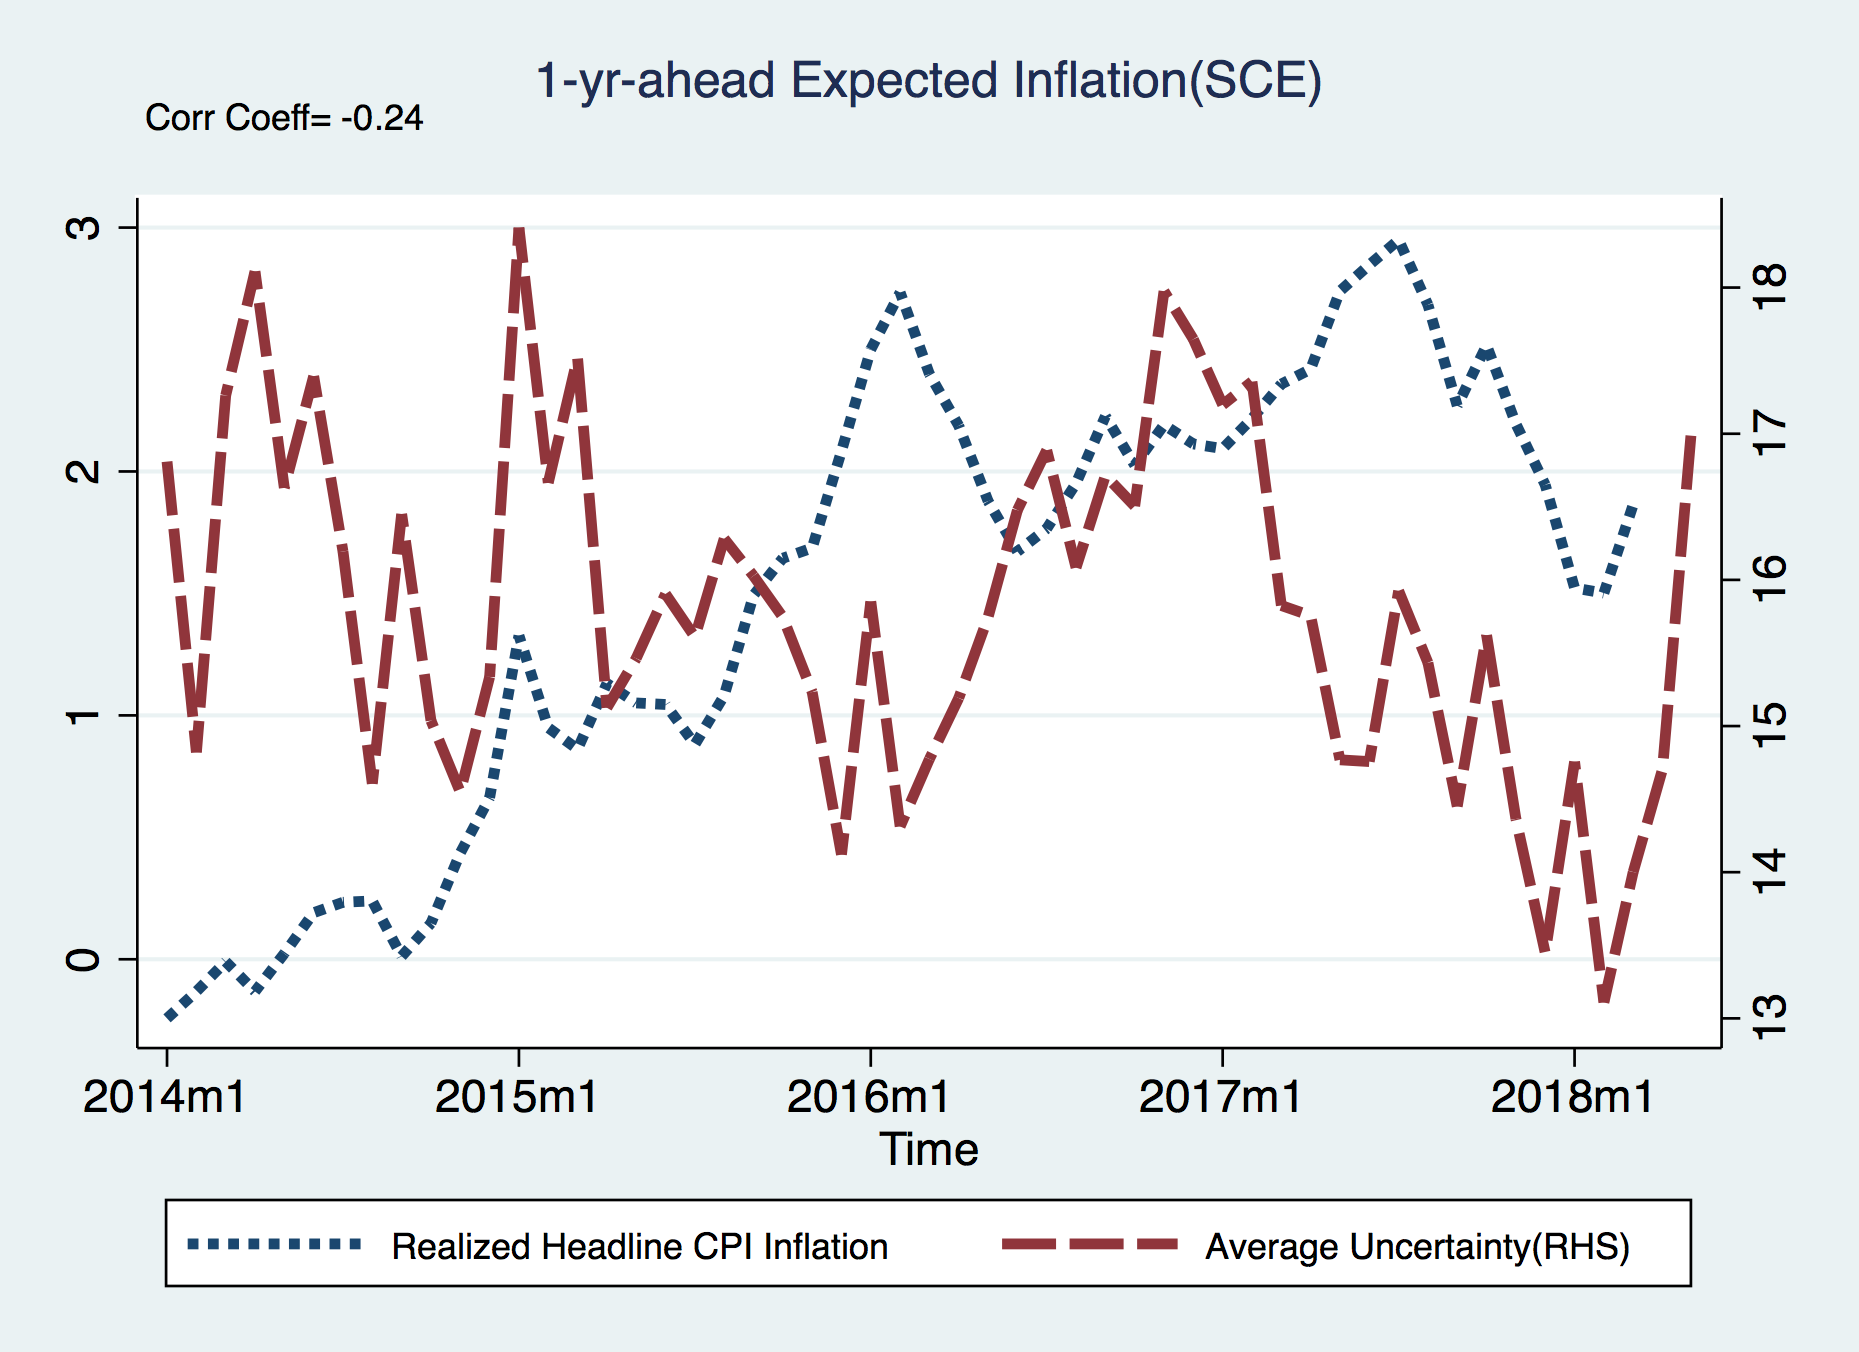
\includegraphics[width=0.3\textwidth]{figuresDraft/Inf1yf_CPIAU_varSCEM.png}
	\end{figure}

\end{frame}


\begin{frame}{Basic patterns: uncertainty and the size of forecast errors}
	\begin{figure}
		\centering
		\label{FEVar}
		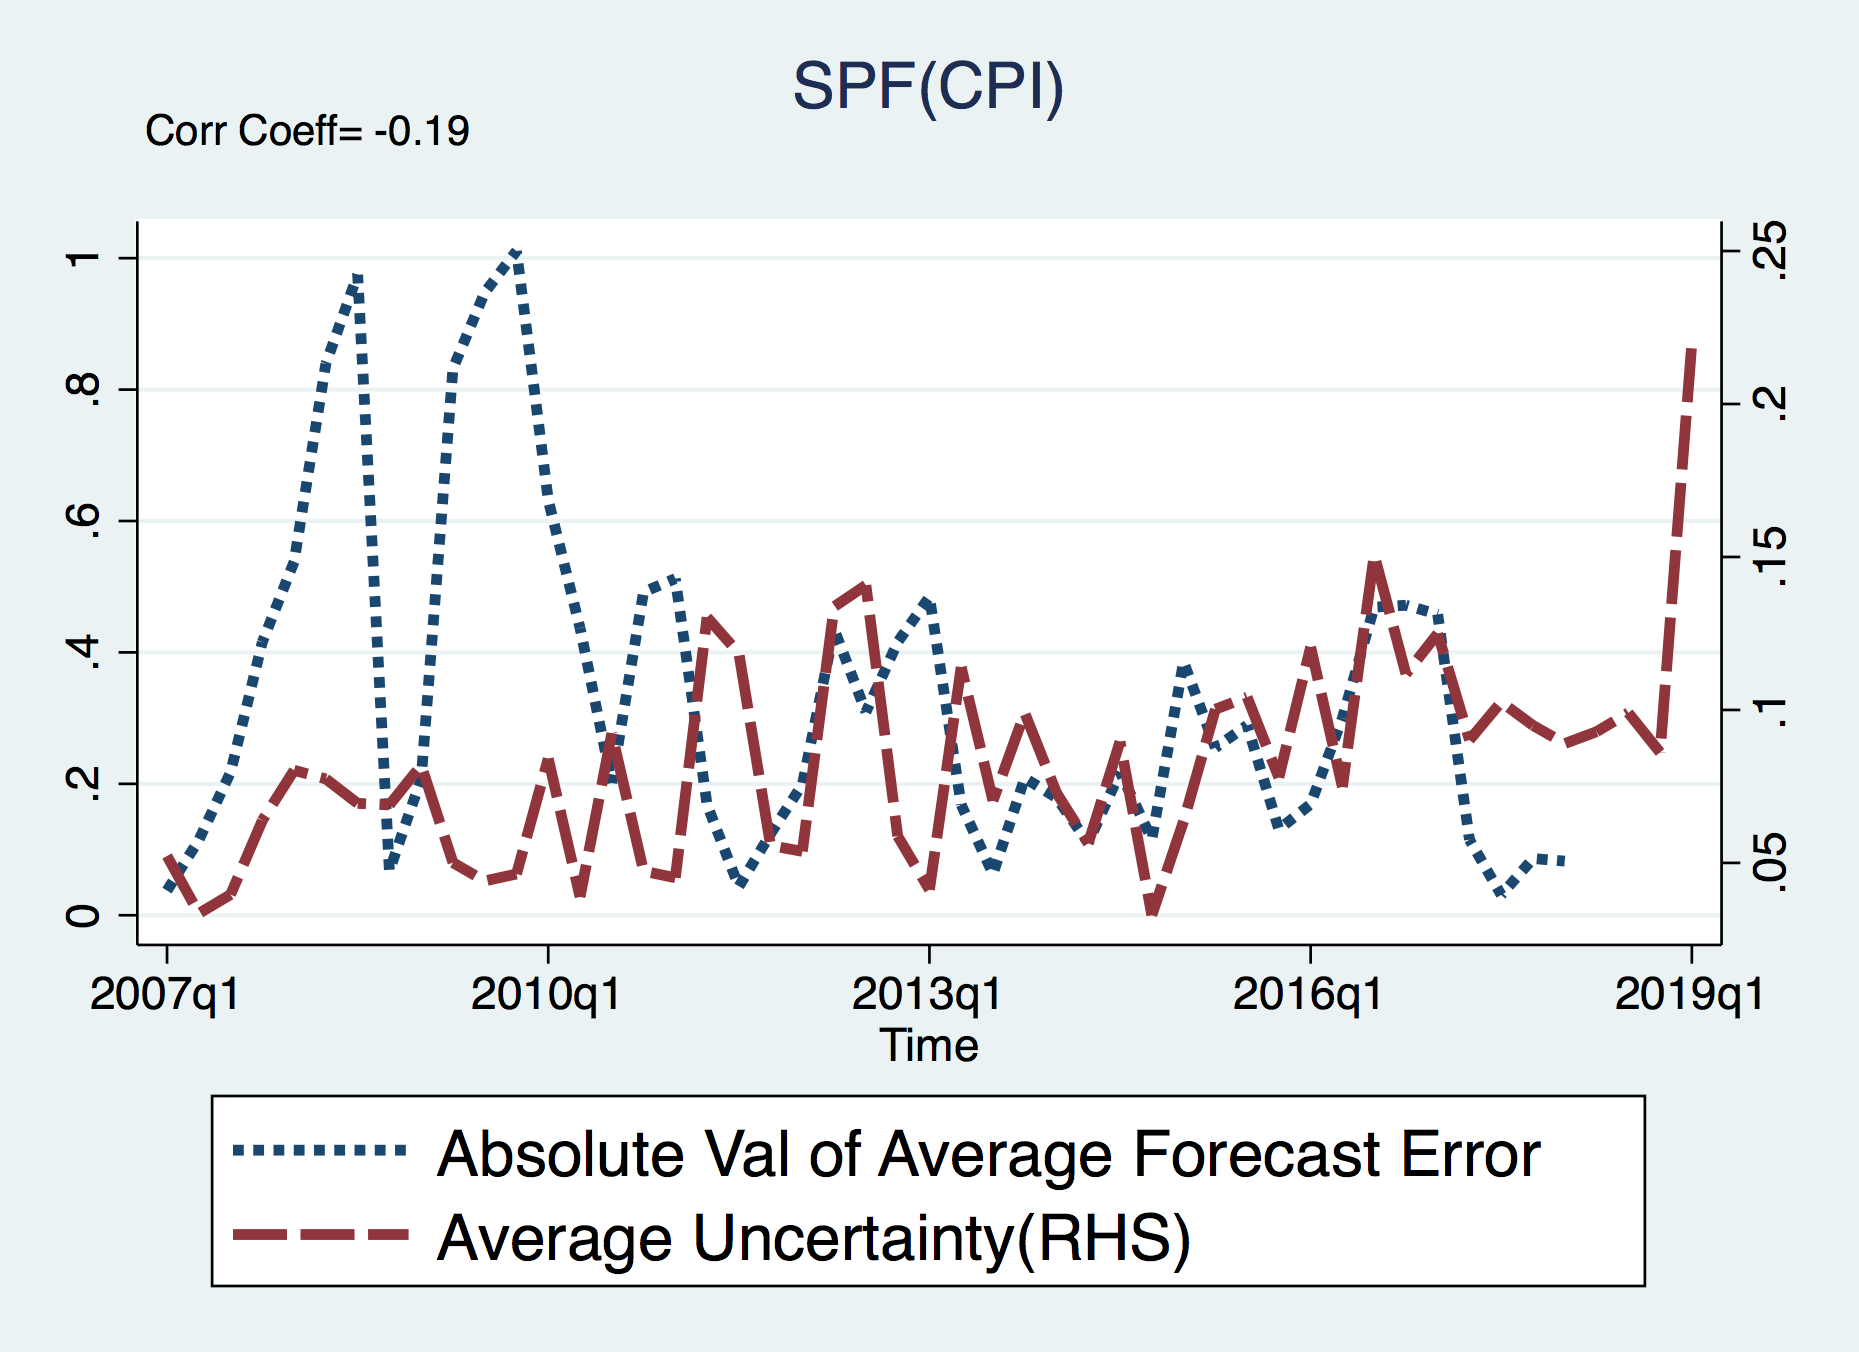
\includegraphics[width=0.3\textwidth]{figuresDraft/SPFCPI_abFE_varSPFCPIQ.png}
		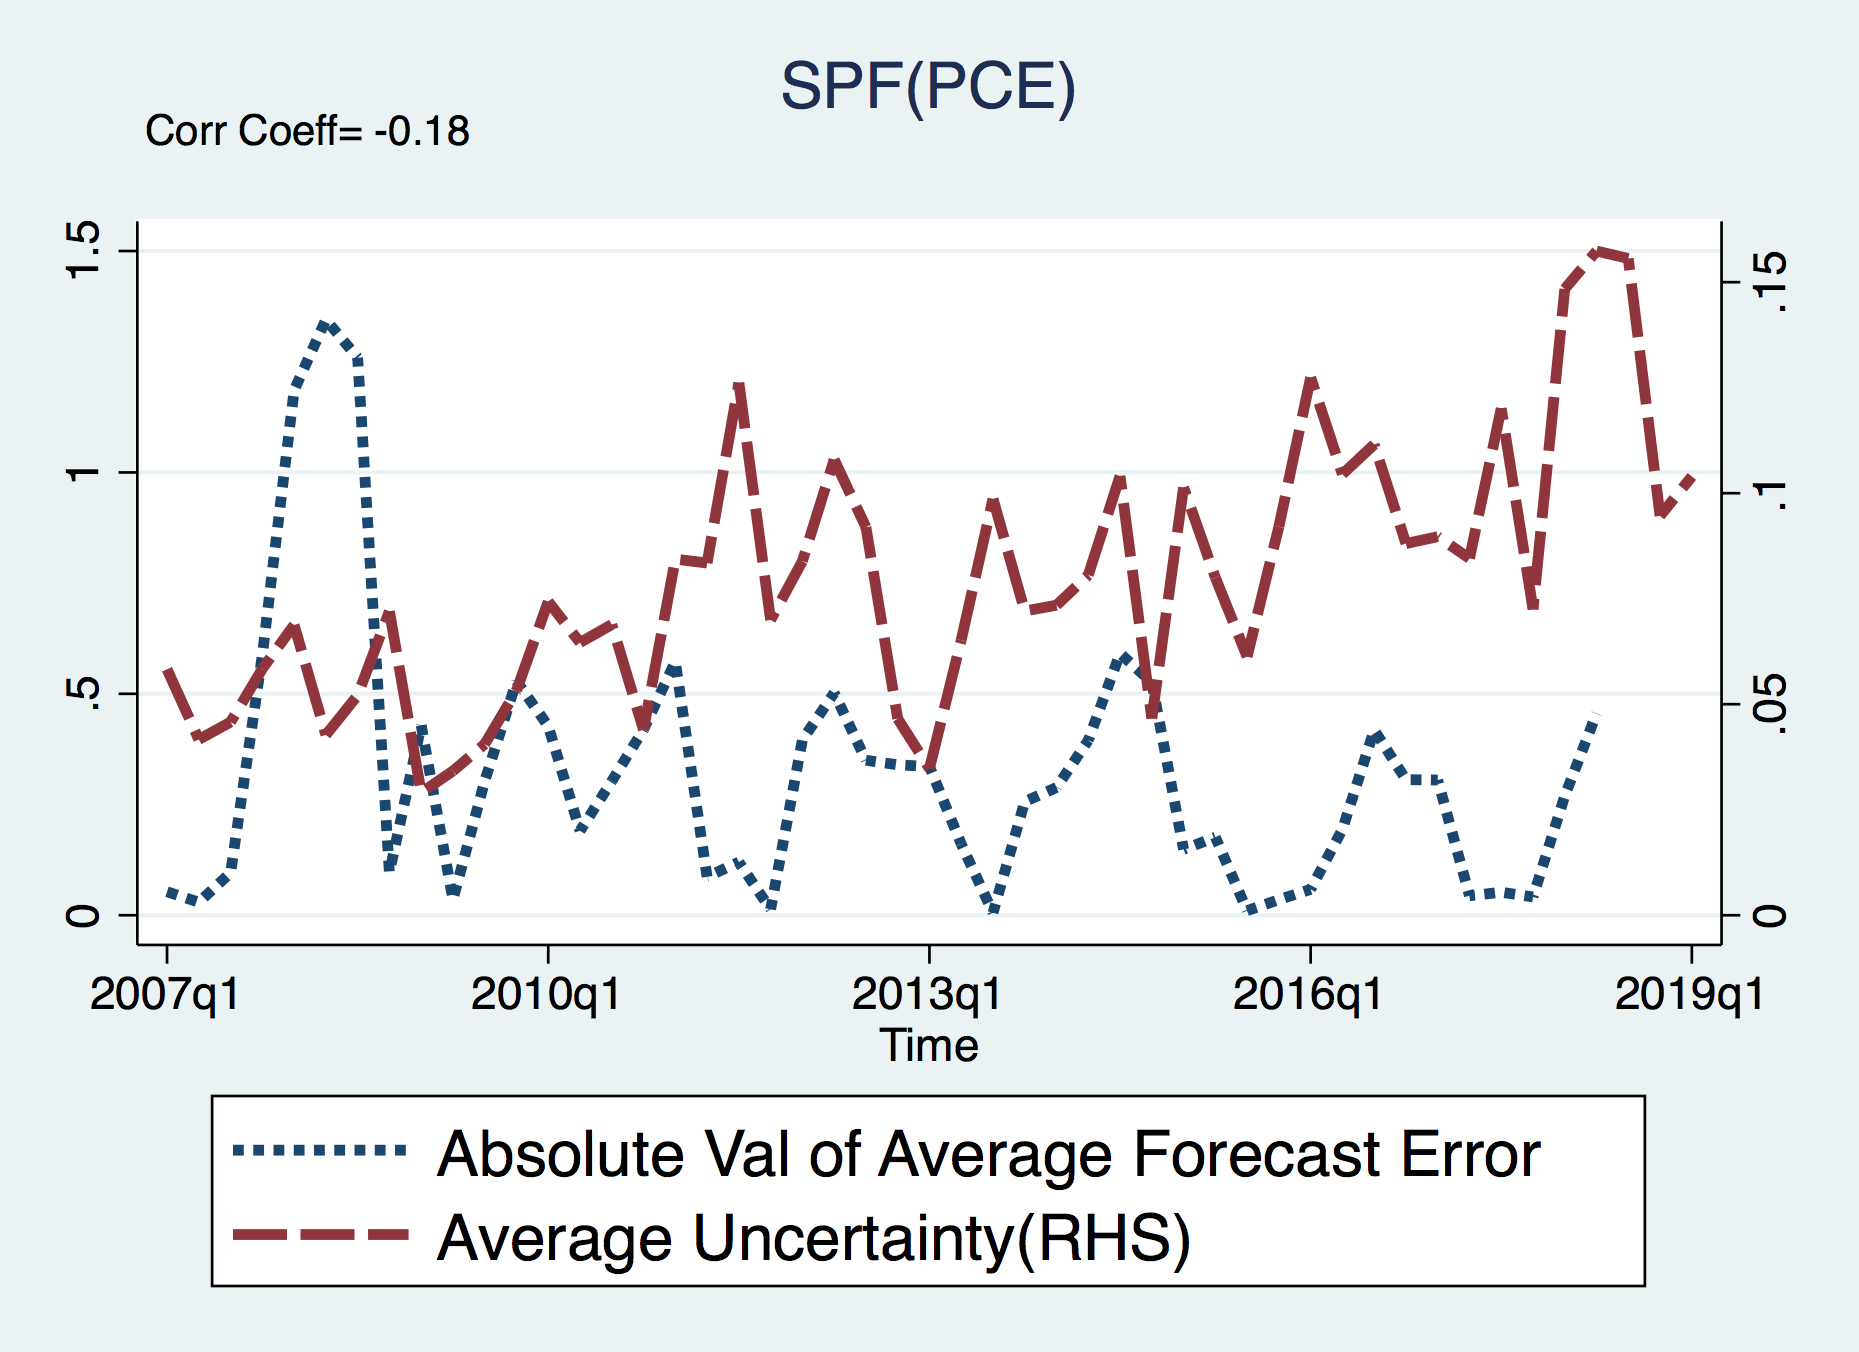
\includegraphics[width=0.3\textwidth]{figuresDraft/SPFPCE_abFE_varSPFPCEQ.png}
		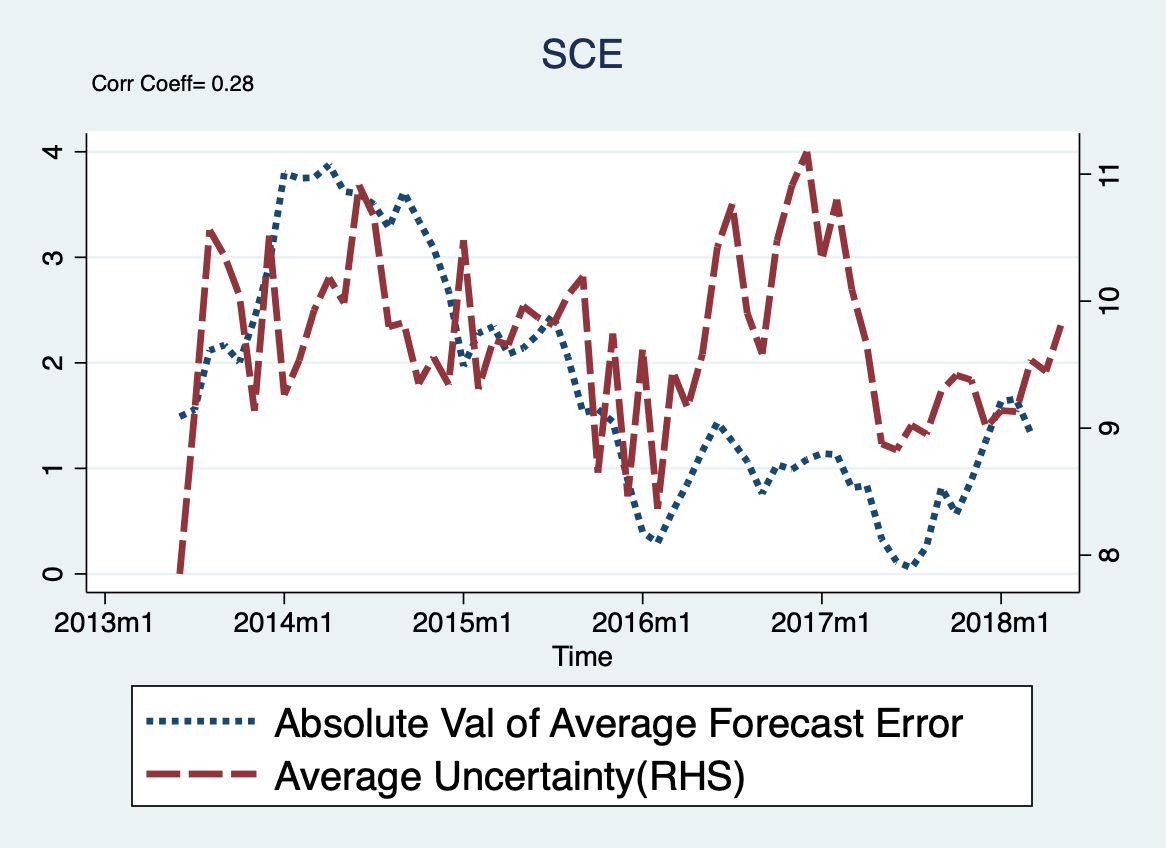
\includegraphics[width=0.3\textwidth]{figuresDraft/SCE_abFE_varSCEM.png}
	\end{figure}
\begin{itemize}
\item no evidence for positive correlation betwen high ex ante uncertainty and ex post forecast errors.
\end{itemize}
\end{frame}

\begin{frame}{Basic patterns: uncertainty and disagreement}
	\begin{figure}
		\centering
		\label{DisgVar}
		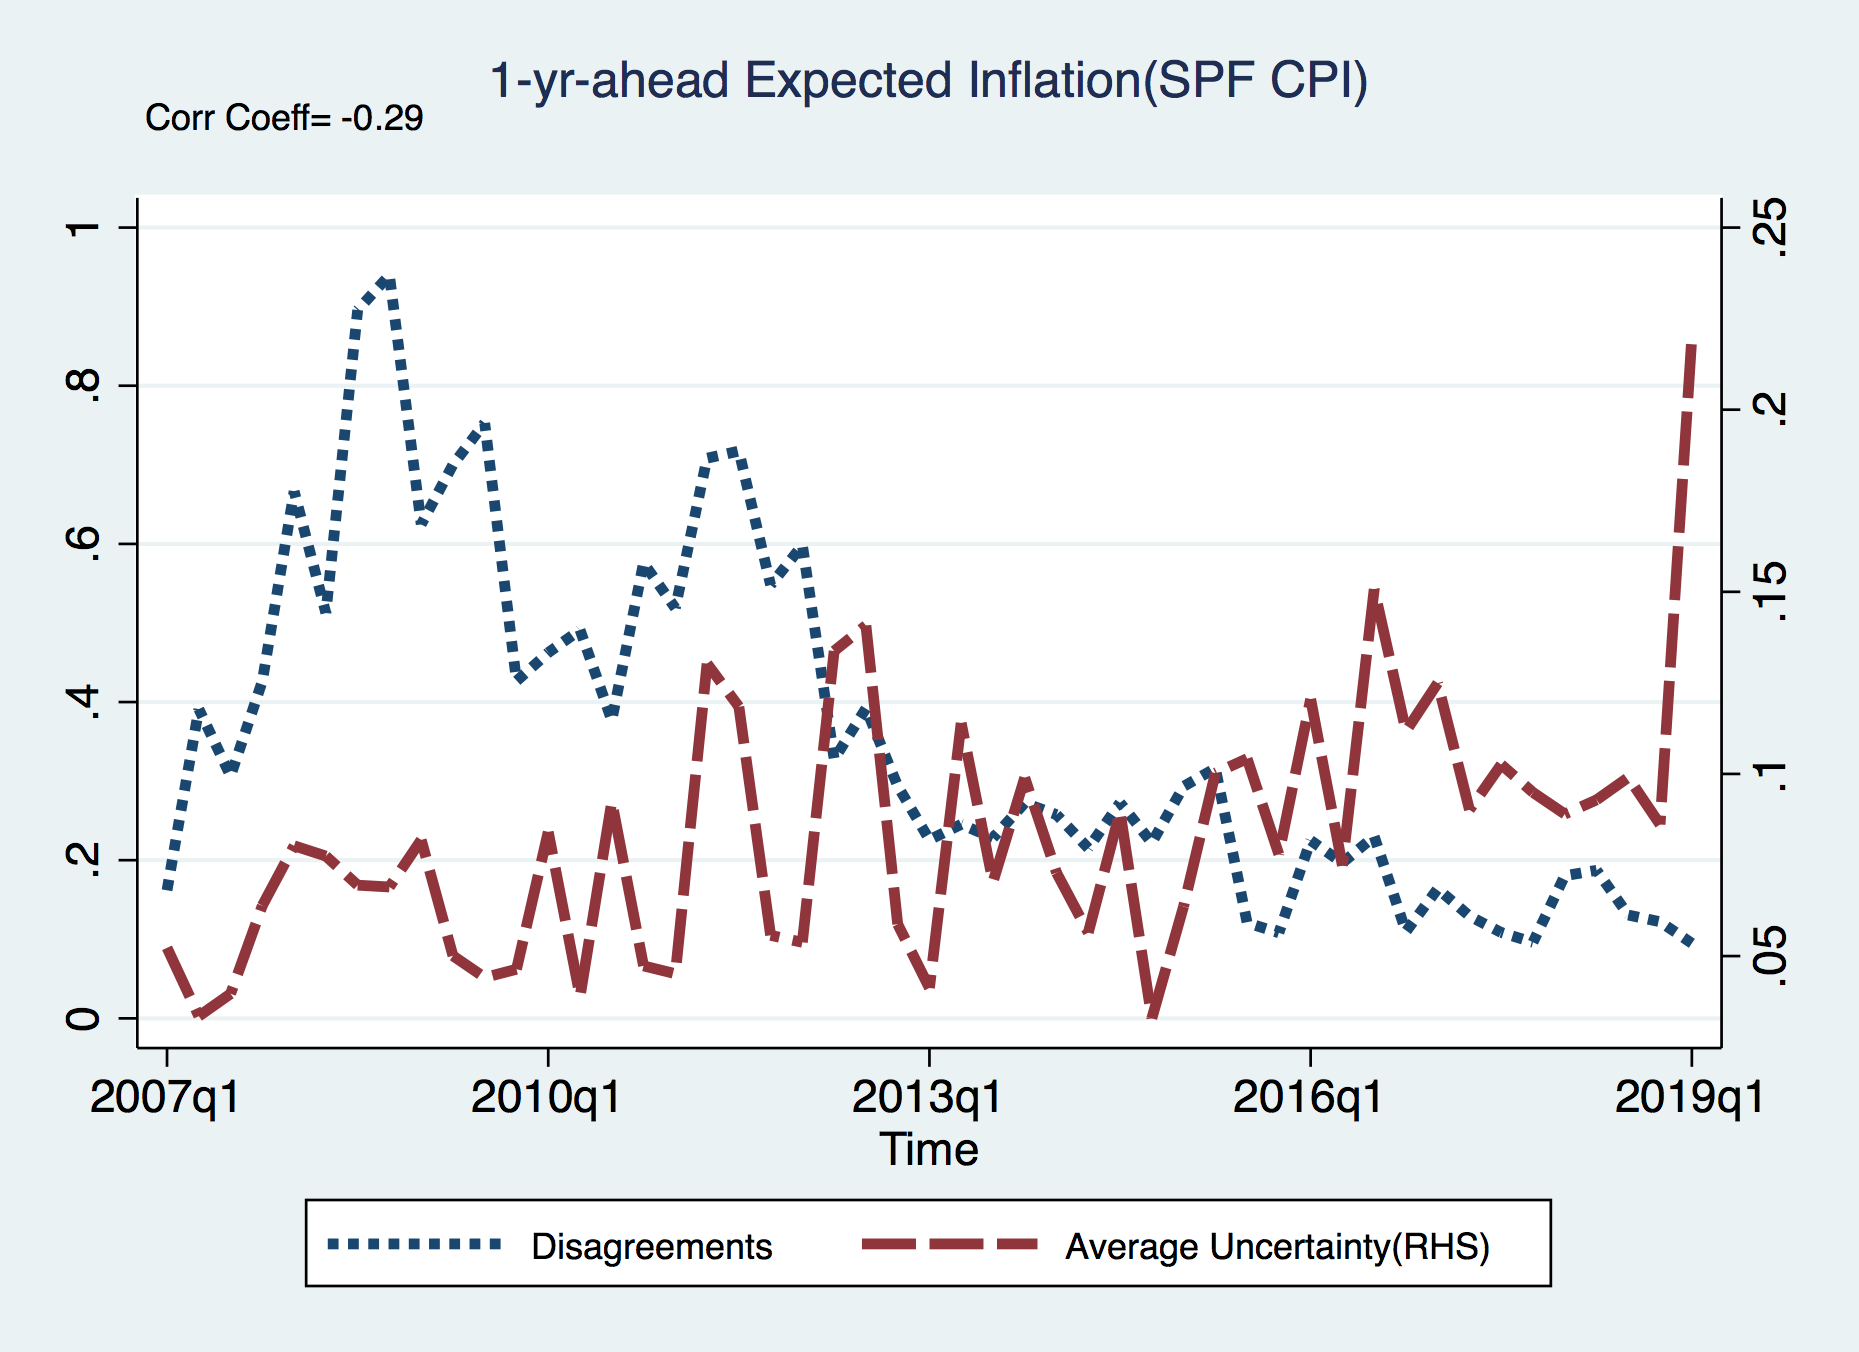
\includegraphics[width=0.3\textwidth]{figuresDraft/CPI_disg_varSPFCPIQ.png}
		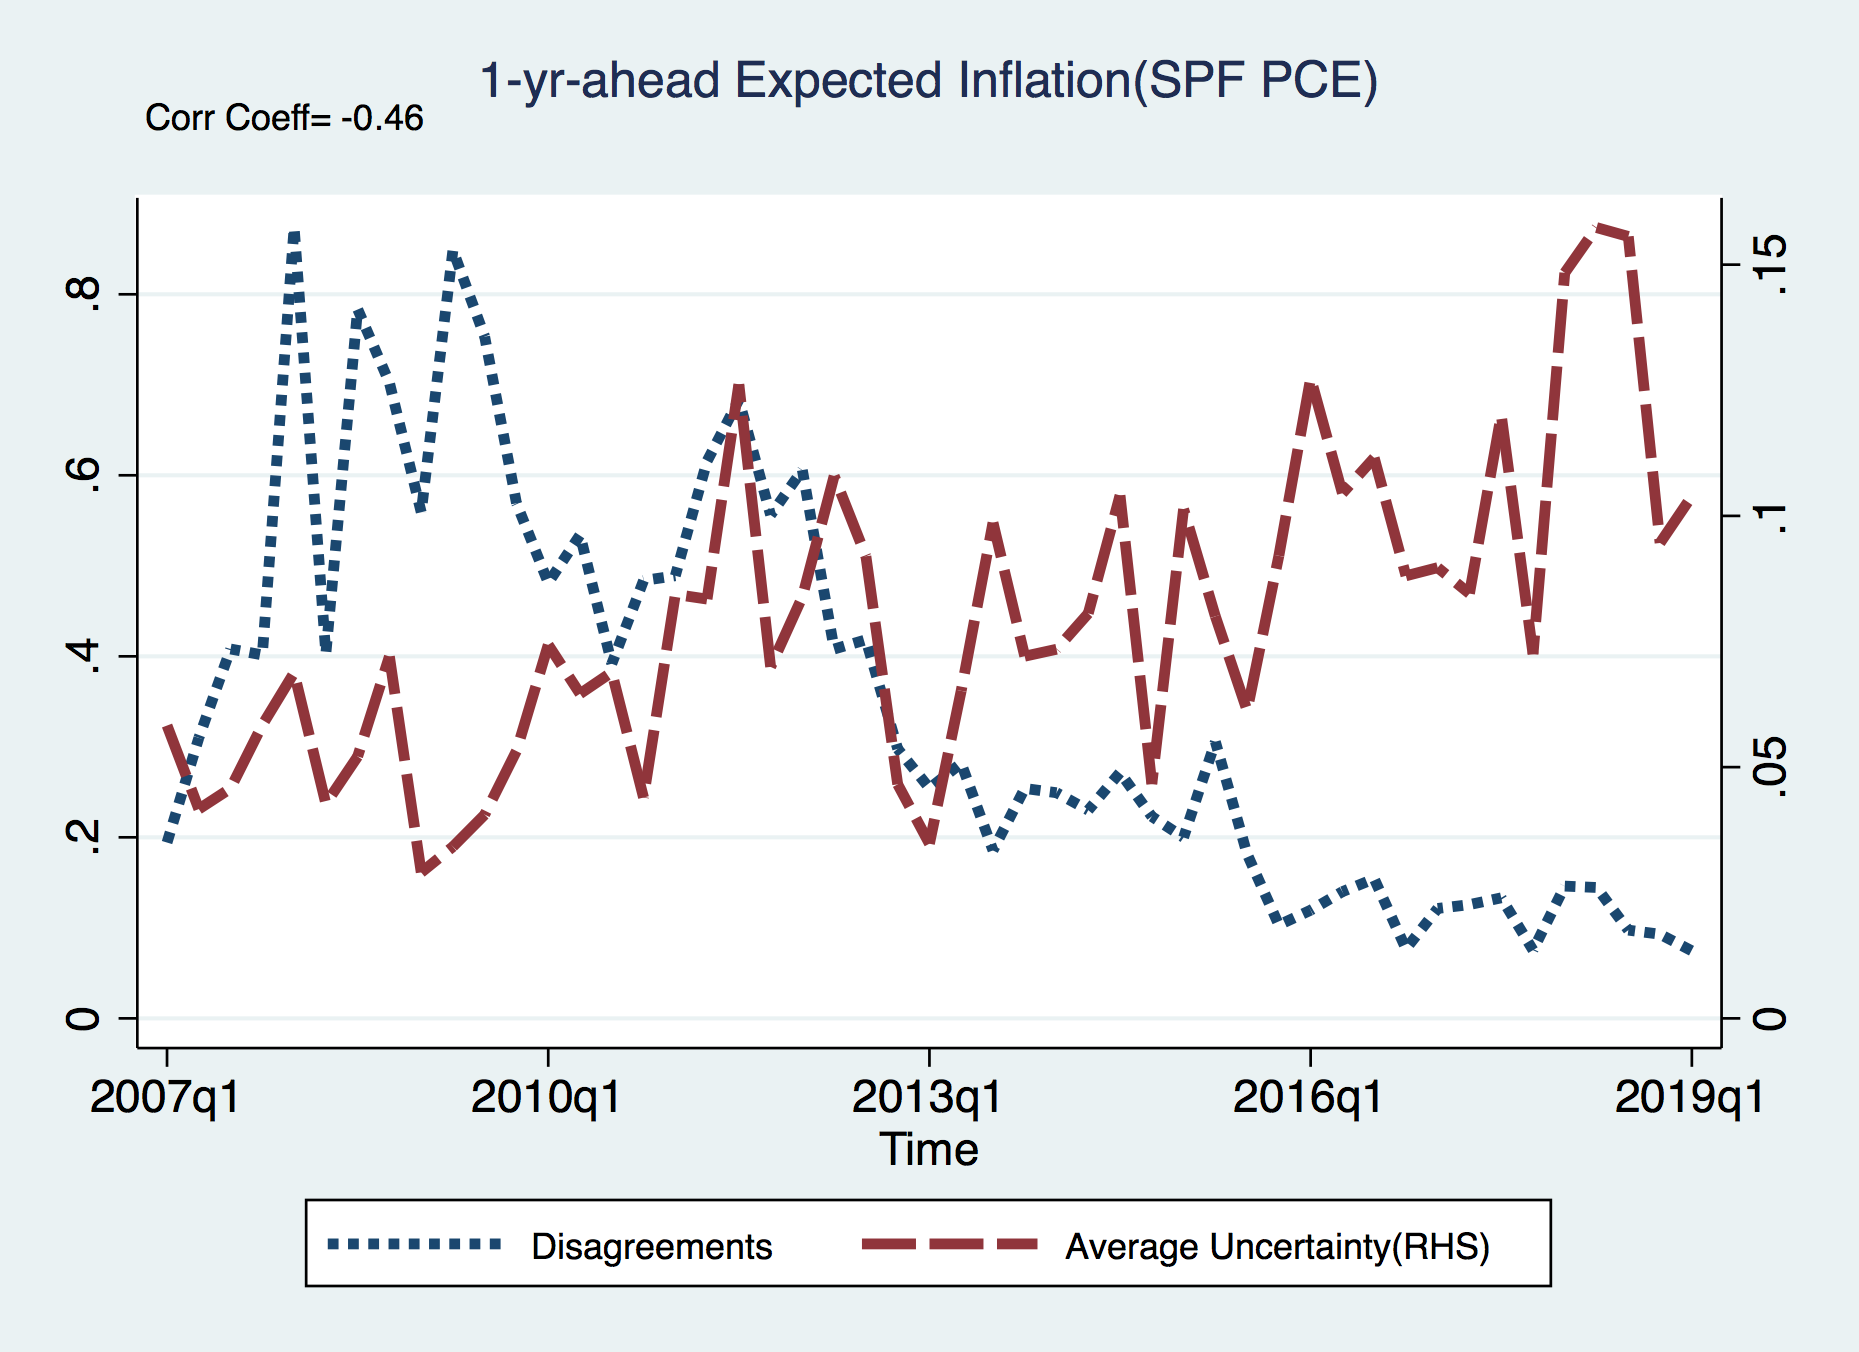
\includegraphics[width=0.3\textwidth]{figuresDraft/PCE_disg_varSPFPCEQ.png}
		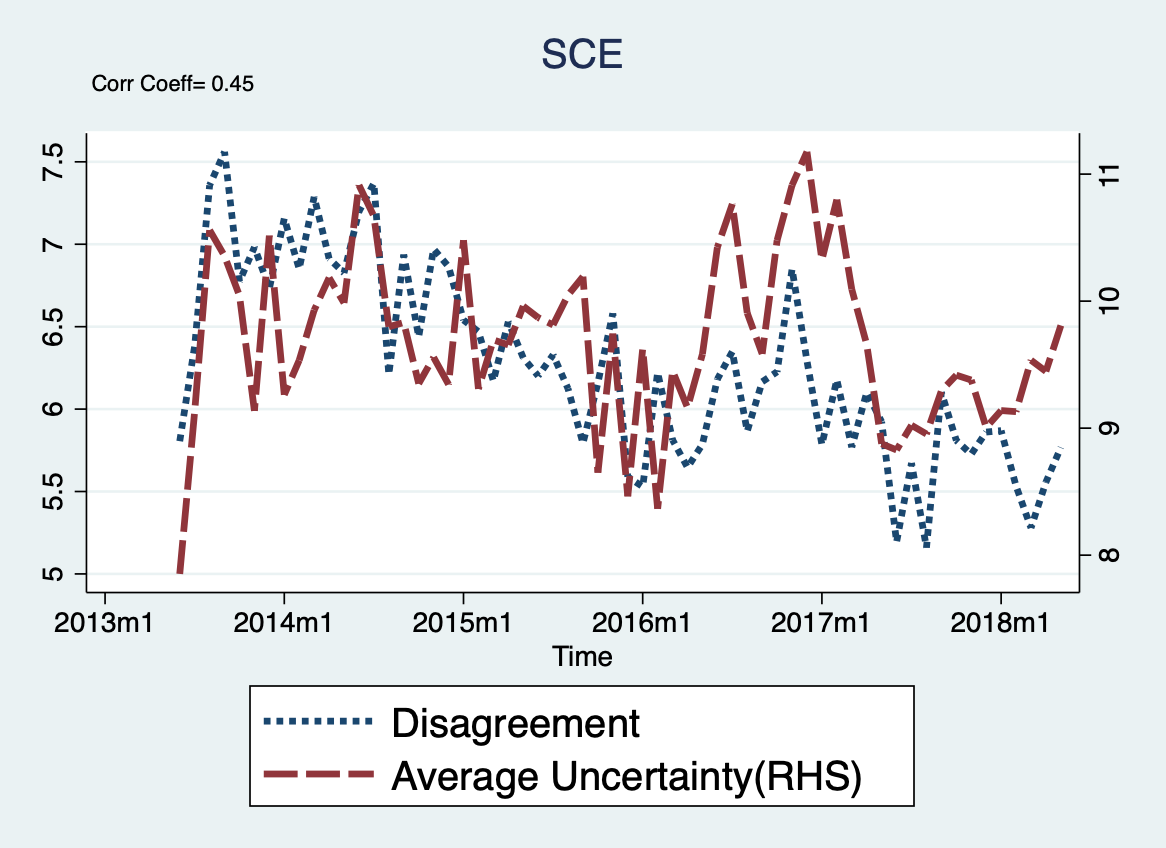
\includegraphics[width=0.3\textwidth]{figuresDraft/Q9_disg_varSCEM.png}
	\end{figure}
\begin{itemize}
	\item uncertainty are not the same as disagreement for professionals 
\end{itemize}
\end{frame}

\begin{frame}{Basic patterns: summary}
	\begin{itemize}
		\item uncertainty varies across time 
		\item uncertainty contains different information from widely  proxies such as disagreement and forecast error
	\end{itemize}
\end{frame}

\section{Theory}

\begin{frame}{AR(1) model of inflation}
	

\begin{itemize}
	
\item 	\textbf{Inflation process}	
	$$y_{t} = \rho y_{t-1} + \omega_t  $$ 
	$$\omega_t \sim N(0,\sigma^2_{\omega})$$

\item \textbf{Uncertainty}
		\begin{itemize}
			\item FIRE: time-invariant 
			\begin{eqnarray*}\label{VarREPop}
				\overline{Var}^*_{t+h|t} = \sum^{h}_{s=1}\rho^{2s} \sigma^2_{\omega}
			\end{eqnarray*}
			
			\item SE: time-invariant 
			\begin{eqnarray*}\label{VarSEPopRE}
				\overline{Var}^{se}_{t+h|t} = \sum^{+\infty}_{\tau =0} \lambda (1-\lambda)^\tau \overline{Var}^*_{t+h|t-\tau}
			\end{eqnarray*}
			
			\item NI: time-variant but quantitatively tiny due to highly efficient Kalman gain
			
			\begin{eqnarray*}\label{VarNIPopRE}
				\overline{Var}^{ni}_{t+h|t} = \rho^{2h} \overline{Var}^{ni}_{t|t} + \overline{Var}^*_{t+h|t}
			\end{eqnarray*}
		\end{itemize}
		
	\end{itemize}
	
\end{frame}

\begin{frame}{Stocastic volatility (UCSV) inflation process (\citet{stock2007has})}

\begin{itemize}
\item \textbf{Inflation process}
\begin{eqnarray*}
\begin{split}
& y_t = \theta_t + \eta_t,\quad \textrm{where } \eta_t =\sigma_{\eta,t} \xi_{\eta,t} \\
& \theta_t = \theta_{t-1} + \epsilon_t, \quad \textrm{where }  \epsilon_t =\sigma_{\epsilon,t} \xi_{\epsilon,t} \\
& \log\sigma^2_{\eta,t} = \log\sigma^2_{\eta,t-1} + \mu_{\eta,t} \\
& \log\sigma^2_{\epsilon,t} = \log\sigma^2_{\epsilon,t-1} + \mu_{\epsilon,t} 
\end{split}
\end{eqnarray*}

\begin{eqnarray*}
\begin{split}
& \xi_t =[\xi_{\eta,t},\xi_{\epsilon,t}] \sim N(0,I_2) \\
& \mu_{t} = [\mu_{\eta,t},\mu_{\epsilon,t}]' \sim N(0,\gamma I_2) 
\end{split}
\end{eqnarray*}
\end{itemize}

\end{frame}


\begin{frame}{UCSV inflation process}
	
	\begin{itemize}
		\item \textbf{Uncertainty}
		\begin{itemize}
			\item FIRE: time-varying  \begin{eqnarray*}\label{VARRESVPop}
			\begin{split}
			\overline{Var}^*_{t+h|t} = \sum_{k=1}^h exp^{- 0.5k\gamma_{\eta}} \sigma^2_{\eta,t}  +  exp^{- 0.5 h \gamma_{\epsilon}} \sigma^2_{\epsilon,t} 
			\end{split} 
			\end{eqnarray*}
			
			\item SE: time-varying 
			\begin{eqnarray*}
		\overline {Var}^{se}_{t+h|t} = \sum^{\infty}_{\tau=0} (1-\lambda)^\tau\lambda\overline{Var}^*_{t+h|t-\tau} 
			\end{eqnarray*}
			
			\item NI (1-step-ahead): time-varying 
		\begin{eqnarray*}
		\overline{Var}^\theta_{t|t-1} = \overline{Var}^\theta_{t-1|t-1} + Var^*_{t|t-1}(y_t) 
		\end{eqnarray*}
			
		\end{itemize}
	\end{itemize}
	
\end{frame}


\section{Estimation}
\begin{frame}{Simulated method of moment estimation}
	
	\begin{eqnarray*}
	\widehat \Omega = \underset{\{\Omega \in \Gamma\} }{argmin} (M_{\textrm{data} } - F^{o}(\Omega, Y)) W  (M_{\textrm{data} } - F^{o}(\Omega, Y))'
	\end{eqnarray*}
	
	\begin{itemize}
		\item  $\Omega$: parameters of the particular $o \in \{{fire}, {se}, {ni},{de},{seni} \} \times \{ar, sv\}$
		\item  $\Gamma$: constraints for the parameter. 
		\item $M_{data}$: data moments
		\item $F$: simulated model moments according to a particular theory $o$, a function of parameters $\Omega$ as well as the $Y$, the real-time data (including history) up till each point of the time $t$. 
		\begin{itemize}
			\item unconditional moments, not specific to time
			\item moments selected from average forecast, variance and autocovariance of forecasts, average diagreement, variance and autovariance of disagreement, average uncertainty, etc. 
		\end{itemize}
		\item  $W$: weight matrix, identity matrix for now 
	\end{itemize}
\end{frame}


\begin{frame}{Estimation procedure and algorithm}
	\begin{enumerate}
		\item for each theory of expectation formation and the inflation process, start with an initial value for the parameter(s) of interest
		\item simulate individual forecasts for a large enough ($N=200$) number of forecasters
		\item compute the average forecast errors, disagreement and average uncertainty across all agents
		\item compute the time-series moments of the average forecast, disagreement, and uncertainty
		\item compute the difference between the simulated moments and the data moments 
		\item keep searching the parameter value until reaching below a threshold of the loss
	\end{enumerate}
\end{frame}


\begin{frame}{Two-step and joint estimation}
	\begin{enumerate}
		\item two-step estimation:  separately estimate inflation process parameters and then parameters of the inflation process
		\begin{itemize}
			\item pros: computationally lighter 
			\item cons: potential misspecification. does not utilize the expectation data to understand inflation process per se.  
		\end{itemize}
		\item joint estimation: targeting both moments of realized inflation series and moments of forecasts to simultaneously estimate both the inflation process and the parameter of expectation formation
		\begin{itemize}
			\item pros: additional information gain from expectations data about inflation process itself
			\item cons: more computation burden  
		\end{itemize}
	\end{enumerate}
\end{frame}


\begin{frame}{Scoring card for a theory of expectation formation}
	To look if the parameter and goodness of fit is robust to 
	\begin{enumerate}
		\item use of different moments in estimation
		\item alternative assumption about the underlying process 
		\item two-step estimation or joint-estimation 
		\item relatively fit with professionals and households  
	\end{enumerate}
\end{frame}

\subsection{AR(1)}

%%%%%%%%%%%%%%%%%%%
\subsubsection{SE}

\begin{frame}{SE parameter estimate}
	\begin{table}
		\centering
		\caption{SMM Estimates of SE}
		\label{SMM_Est_SE_Table}
		\adjustbox{max height=0.5\textheight, max width=\textwidth}{ 
	\begin{tabular}{lllllllllllll}
		\hline 
		0     & 1       & 2       & 3       &     & SE: $\hat\lambda_{SPF}$(Q) & SE: $\hat\lambda_{SPF}$(Q) & SE: $\rho$ & SE: $\sigma$ & SE: $\hat\lambda_{SCE}$(M) & SE: $\hat\lambda_{SCE}$(M) & SE: $\rho$ & SE: $\sigma$ \\
		\hline 
		FEVar & FEATV   &         &         &     & 0.47                       & 0.36                       & 1          & 0.08         & 0.2                        & 0.5                        & 0.84       & 0.25         \\
		FEVar & DisgATV & DisgVar &         &     & 0.47                       & 0.38                       & 1          & 0.1          & 0.21                       & 0.54                       & 0.92       & 0.18         \\
		FEVar & FEATV   & DisgVar & DisgATV & Var & 0.47                       & 0.36                       & 1          & 0.08         & 0.21                       & 0.5                        & 0.84       & 0.25       \\
		\hline 
	\end{tabular}
	}
	\end{table}
	\begin{itemize}
		\item $\lambda$: update rate in SE
	\end{itemize}
\end{frame}



\begin{frame}{Professionals and SEAR}
	\begin{figure}[ht]
		\label{SE_diag_SPF}
		\begin{subfigure}[b]{0.2\textwidth}
			\centering
			\caption{FE}
			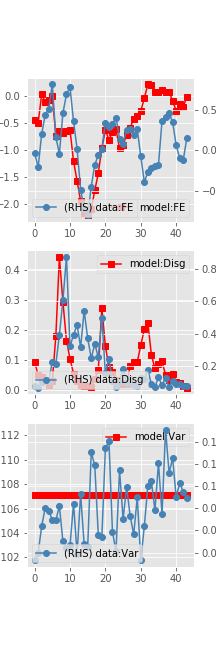
\includegraphics[width=\textwidth, height = 0.8\textheight]{figuresDraft/spf_se_est_diag0.png}
		\end{subfigure}
		\hfill
		\begin{subfigure}[b]{0.2\textwidth}
			\caption{Disg}
			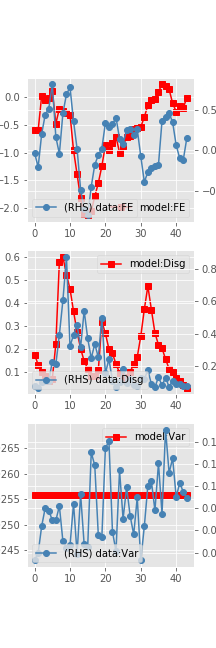
\includegraphics[width=\textwidth, height = 0.8\textheight]{figuresDraft/spf_se_est_diag1.png}
		\end{subfigure}
		\hfill
		\begin{subfigure}[b]{0.2\textwidth}
			\caption{FE/Disg}
			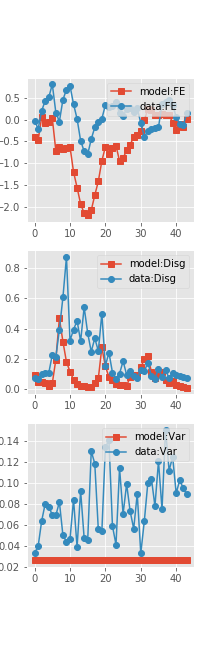
\includegraphics[width=\textwidth, height = 0.8\textheight]{figuresDraft/spf_se_est_diag2.png}
		\end{subfigure}
	\end{figure}
\end{frame}


\begin{frame}{Professionals and SEAR: joint estimation}
	\begin{figure}[ht]
		\label{SE_diag_SPF_joint}
		\begin{subfigure}[b]{0.2\textwidth}
			\centering
			\caption{FE}
			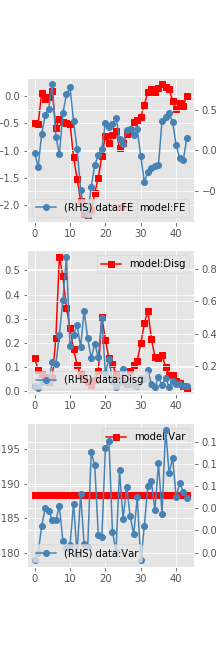
\includegraphics[width=\textwidth, height = 0.8\textheight]{figuresDraft/spf_se_est_joint_diag0.png}
		\end{subfigure}
		\hfill
		\begin{subfigure}[b]{0.2\textwidth}
			\caption{Disg}
			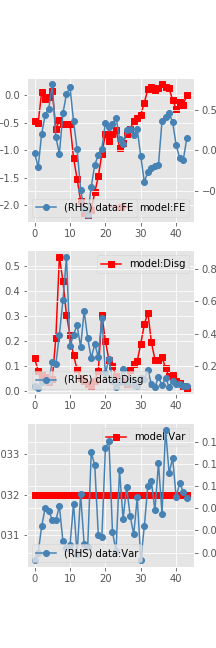
\includegraphics[width=\textwidth, height = 0.8\textheight]{figuresDraft/spf_se_est_joint_diag1.png}
		\end{subfigure}
		\hfill
		\begin{subfigure}[b]{0.2\textwidth}
			\caption{FE/Disg}
			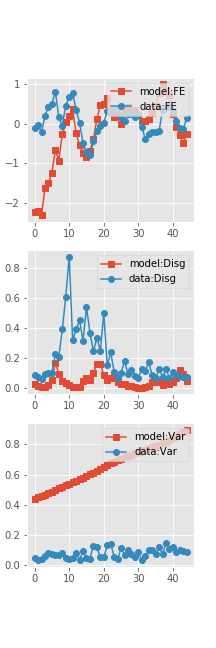
\includegraphics[width=\textwidth, height = 0.8\textheight]{figuresDraft/spf_se_est_joint_diag2.png}
		\end{subfigure}
	\end{figure}
\end{frame}


\begin{frame}{Households and SEAR}
	\begin{figure}[ht]
		\label{SE_diag_SCE}
		\begin{subfigure}[b]{0.2\textwidth}
			\centering
			\caption{FE}
			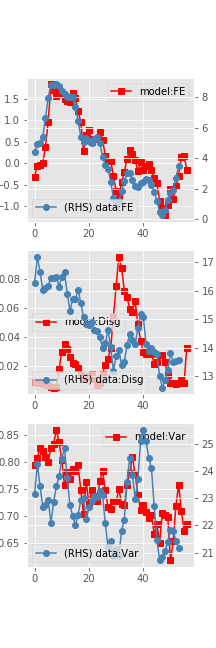
\includegraphics[width=\textwidth, height = 0.8\textheight]{figuresDraft/sce_se_est_diag0.png}
		\end{subfigure}
		\hfill
		\begin{subfigure}[b]{0.2\textwidth}
			\caption{Disg}
			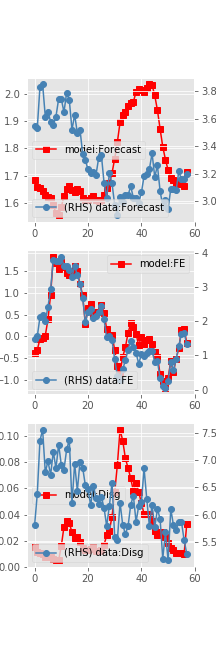
\includegraphics[width=\textwidth, height = 0.8\textheight]{figuresDraft/sce_se_est_diag1.png}
		\end{subfigure}
		\hfill
	\begin{subfigure}[b]{0.2\textwidth}
		\caption{FE/Disg}
		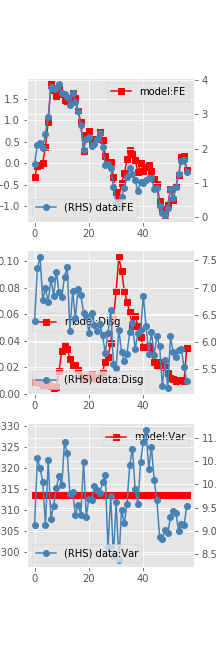
\includegraphics[width=\textwidth, height = 0.8\textheight]{figuresDraft/sce_se_est_diag2.png}
	\end{subfigure}
	\end{figure}
\end{frame}


\begin{frame}{Households and SEAR: joint estimates}
	\begin{figure}[ht]
		\label{SE_diag_SCE_joint}
		\begin{subfigure}[b]{0.2\textwidth}
			\centering
			\caption{FE}
			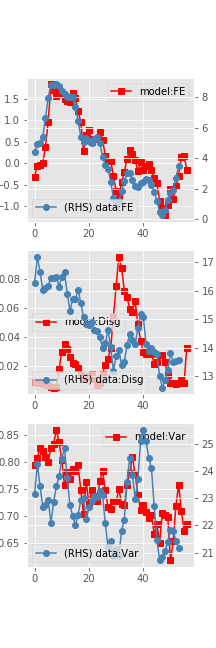
\includegraphics[width=\textwidth, height = 0.8\textheight]{figuresDraft/sce_se_est_diag0.png}
		\end{subfigure}
		\hfill
		\begin{subfigure}[b]{0.2\textwidth}
			\caption{Disg}
			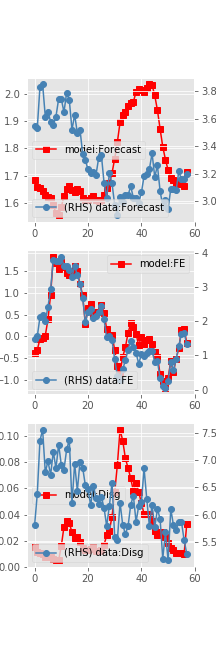
\includegraphics[width=\textwidth, height = 0.8\textheight]{figuresDraft/sce_se_est_diag1.png}
		\end{subfigure}
		\hfill
		\begin{subfigure}[b]{0.2\textwidth}
			\caption{FE/Disg}
			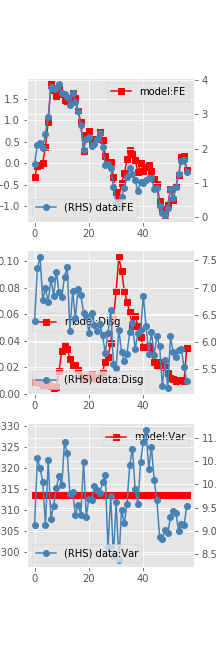
\includegraphics[width=\textwidth, height = 0.8\textheight]{figuresDraft/sce_se_est_diag2.png}
		\end{subfigure}
	\end{figure}
\end{frame}

%%%%%%%%%%%%%%%%%%%%%%

\subsubsection{DE}

\begin{frame}{DE parameter estimate}
	\begin{table}
		\centering
		\caption{SMM Estimates of DE}
		\label{SMM_Est_DE_Table}
		\adjustbox{max height=0.5\textheight, max width=\textwidth}{ 
		\begin{tabular}{lllllllllllllllllll}
			\hline 
			0  & 1     & 2     & 3    & 4       & 5       & 6   & DE: $\theta_{SPF}$ & DE: $\sigma_{\theta,SPF}$ & DE: $\theta_{SPF}$ & DE: $\sigma_{\theta,SPF}$ & DE: $\rho$ & DE: $\sigma$ & DE: $\theta_{SCE}$ & DE: $\sigma_{\theta,SCE}$ & DE: $\theta_{SCE}$ & DE: $\sigma_{\theta_SCE}$ & DE: $\rho$ & DE: $\sigma$ \\
			\hline 
			FE & FEVar & FEATV &      &         &         &     & -0.23              & 0.22                      & NA                 & NA                        & NA         & NA           & 9.35               & 10.65                     & 0.82               & 0.85                      & 1          & 0            \\
			FE & FEVar & FEATV & Disg & DisgVar & DisgATV &     & -0.26              & 1.41                      & -0.14              & 1.44                      & 0.99       & 0.16         & 8.2                & 9.52                      & 4.79               & 4.59                      & 0.58       & 0.55         \\
			FE & FEVar & FEATV & Disg & DisgVar & DisgATV & Var & -0.24              & 1.43                      & -0.17              & 1.44                      & 0.99       & 0.16         & 4.78               & 3.01                      & NA                 & NA                        & NA         & NA          \\
			\hline 
		\end{tabular}
		}
	\end{table}
	\begin{itemize}
	\item $\theta$: representativeness parameter, $\theta>0$ according to DE. 
	\item $\sigma_\theta$: dispersion of representativeness across population
\end{itemize}
\end{frame}



\begin{frame}{Professionals and DEAR}
	\begin{figure}[ht]
		\label{DE_diag_SPF}
		\begin{subfigure}[b]{0.2\textwidth}
			\centering
			\caption{FE}
			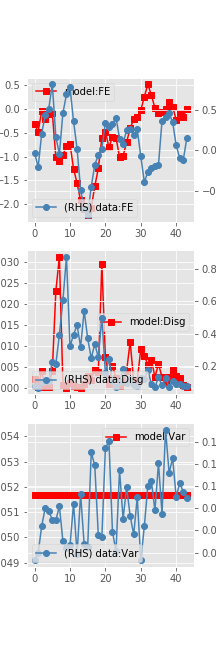
\includegraphics[width=\textwidth, height = 0.8\textheight]{figuresDraft/spf_de_est_diag0.png}
		\end{subfigure}
		\hfill
		\begin{subfigure}[b]{0.2\textwidth}
			\caption{Disg}
			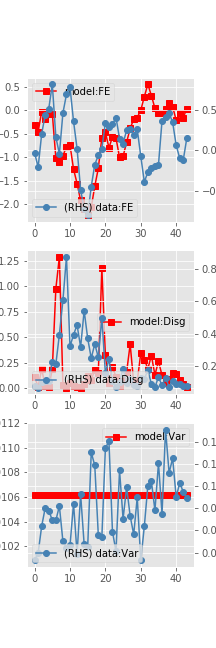
\includegraphics[width=\textwidth, height = 0.8\textheight]{figuresDraft/spf_de_est_diag1.png}
		\end{subfigure}
		\hfill
		\begin{subfigure}[b]{0.2\textwidth}
			\caption{FE/Disg}
			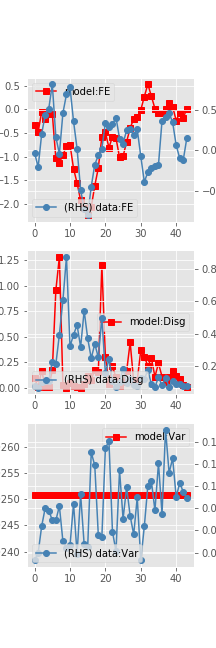
\includegraphics[width=\textwidth, height = 0.8\textheight]{figuresDraft/spf_de_est_diag2.png}
		\end{subfigure}
	\end{figure}
\end{frame}



\begin{frame}{Professionals and DEAR: joint estimate}
	\begin{figure}[ht]
		\label{DE_diag_joint_SPF}
		\begin{subfigure}[b]{0.2\textwidth}
			\centering
			\caption{FE}
			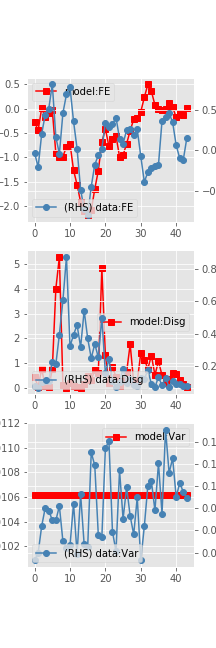
\includegraphics[width=\textwidth, height = 0.8\textheight]{figuresDraft/spf_de_est_joint_diag0.png}
		\end{subfigure}
		\hfill
		\begin{subfigure}[b]{0.2\textwidth}
			\caption{Disg}
			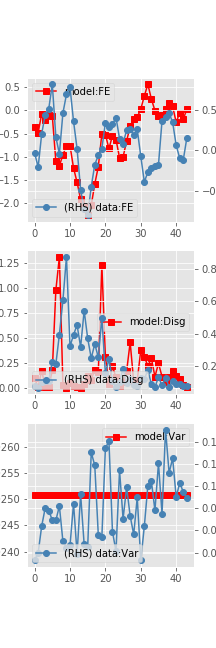
\includegraphics[width=\textwidth, height = 0.8\textheight]{figuresDraft/spf_de_est_joint_diag1.png}
		\end{subfigure}
		\hfill
		\begin{subfigure}[b]{0.2\textwidth}
			\caption{FE/Disg}
			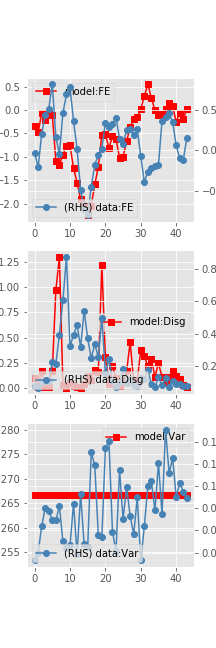
\includegraphics[width=\textwidth, height = 0.8\textheight]{figuresDraft/spf_de_est_joint_diag2.png}
		\end{subfigure}
	\end{figure}
\end{frame}



\begin{frame}{Households and DEAR}
	\begin{figure}[ht]
		\label{DE_diag_SCE}
		\begin{subfigure}[b]{0.2\textwidth}
			\centering
			\caption{FE}
			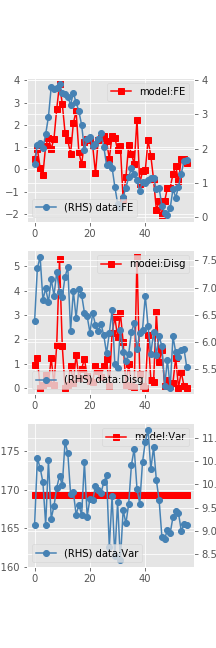
\includegraphics[width=\textwidth, height = 0.8\textheight]{figuresDraft/sce_de_est_diag0.png}
		\end{subfigure}
		\hfill
		\begin{subfigure}[b]{0.2\textwidth}
			\caption{FE/Disg}
			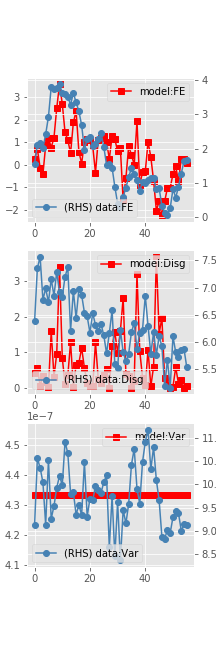
\includegraphics[width=\textwidth, height = 0.8\textheight]{figuresDraft/sce_de_est_diag1.png}
		\end{subfigure}
		\hfill
		\begin{subfigure}[b]{0.2\textwidth}
			\caption{FE/Disg/Var}
			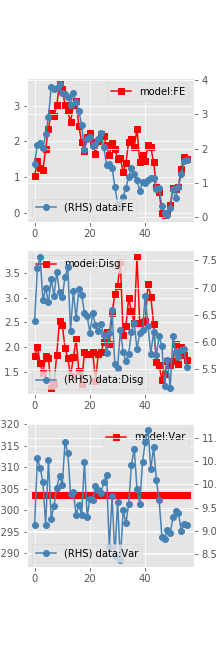
\includegraphics[width=\textwidth, height = 0.8\textheight]{figuresDraft/sce_de_est_diag2.png}
		\end{subfigure}
	\end{figure}
\end{frame}


\begin{frame}{Households and DEAR: joint estimates}
	\begin{figure}[ht]
		\label{DE_diag_joint_SCE}
		\begin{subfigure}[b]{0.2\textwidth}
			\centering
			\caption{FE}
			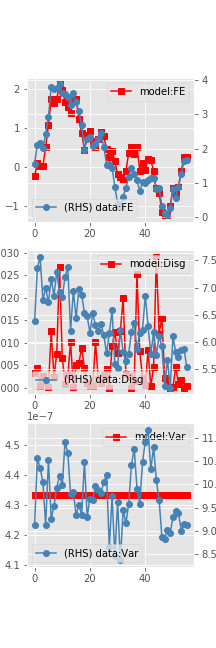
\includegraphics[width=\textwidth, height = 0.8\textheight]{figuresDraft/sce_de_est_joint_diag0.png}
		\end{subfigure}
		\hfill
		\begin{subfigure}[b]{0.2\textwidth}
			\caption{FE/Disg}
			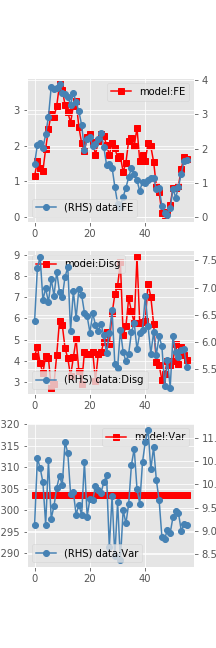
\includegraphics[width=\textwidth, height = 0.8\textheight]{figuresDraft/sce_de_est_joint_diag1.png}
		\end{subfigure}
		\hfill
		\begin{subfigure}[b]{0.2\textwidth}
			\caption{FE/Disg/Var}
			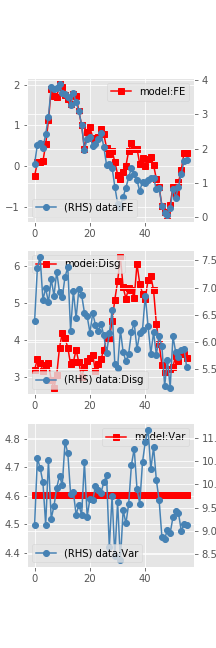
\includegraphics[width=\textwidth, height = 0.8\textheight]{figuresDraft/sce_de_est_joint_diag2.png}
		\end{subfigure}
	\end{figure}
\end{frame}


%%%%%%%%%%%%%%%%%%%
\subsubsection{NI}


\begin{frame}{NIAR parameters}
	\begin{table}
		\centering
		\caption{SMM Estimates of NI}
		\label{SMM_Est_NI_Table}
		\adjustbox{max height=0.5\textheight, max width=\textwidth}{ 
			\begin{tabular}{lllllllllllllllll}
				\hline 
				0     & 1     & 2       & 3       & 4   & NI: $\hat\sigma_{pb,SPF}$ & $\hat\sigma_{pr,SPF}$ & NI: $\hat\sigma_{pb,SPF}$ & $\hat\sigma_{pr,SPF}$ & NI: $\rho$ & NI: $\sigma$ & NI: $\hat\sigma_{pb,SCE}$ & $\hat\sigma_{pr,SCE}$ & NI: $\hat\sigma_{pb,SCE}$ & $\hat\sigma_{pr,SCE}$ & NI: $\rho$ & NI: $\sigma$ \\
				\hline 
				FEVar & FEATV &         &         &     & 0.09                      & 2.77                  & 0.093                     & 1.408                 & 0.911      & 0.422        & 3.4                       & 15.4                  & 3.397                     & 15.395                & 0.997      & 0.027        \\
				FEVar & FEATV & DisgVar & DisgATV &     & 0.09                      & 2.77                  & 0.093                     & 1.408                 & 0.911      & 0.422        & 3.4                       & 15.4                  & 3.397                     & 15.395                & 0.997      & 0.027        \\
				FEVar & FEATV & DisgVar & DisgATV & Var & 0.14                      & 3.85                  & 0.133                     & 1.359                 & 0.911      & 0.422        & 4.9                       & 22.4                  & 4.860                     & 22.367                & 0.997      & 0.027       \\
				\hline 
			\end{tabular}
	}
	\end{table}	
	\begin{itemize}
		\item $\sigma_{pb}$: noisiness of public signals in NI
		\item $\sigma_{pr}$: noisiness of private signals in NI
	\end{itemize}
\end{frame}


\begin{frame}{Professionals and NIAR}
	\begin{figure}[ht]
		\label{NI_diag_SPF}
		\begin{subfigure}[b]{0.2\textwidth}
			\centering
			\caption{FE}
			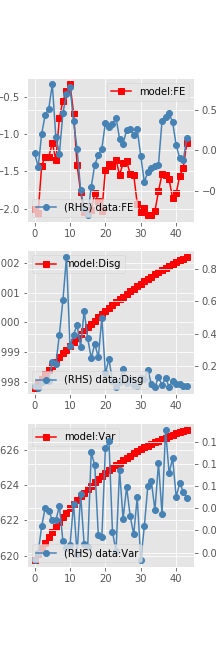
\includegraphics[width=\textwidth, height = 0.8\textheight]{figuresDraft/spf_ni_est_diag0.png}
		\end{subfigure}
		\hfill
		\begin{subfigure}[b]{0.2\textwidth}
			\caption{Disg}
			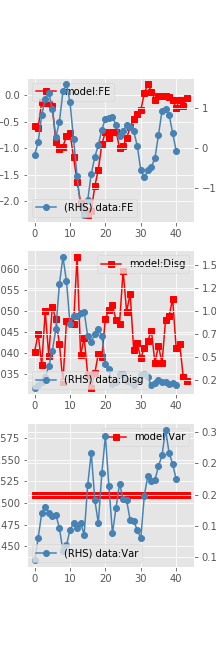
\includegraphics[width=\textwidth, height = 0.8\textheight]{figuresDraft/spf_ni_est_diag1.png}
		\end{subfigure}
		\hfill
		\begin{subfigure}[b]{0.2\textwidth}
			\caption{FE/Disg/Var}
			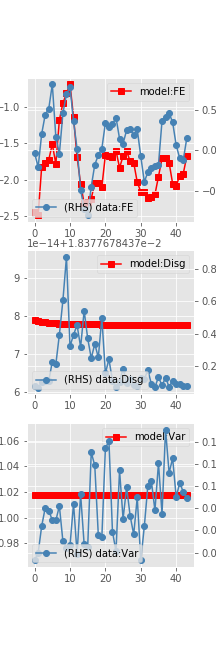
\includegraphics[width=\textwidth, height = 0.8\textheight]{figuresDraft/spf_ni_est_diag2.png}
		\end{subfigure}
	\end{figure}
	\end{frame}


\begin{frame}{Professionals and NIAR: joint estimates}
	\begin{figure}[ht]
		\label{NI_diag_SPF_joint}
		\begin{subfigure}[b]{0.2\textwidth}
			\centering
			\caption{FE}
			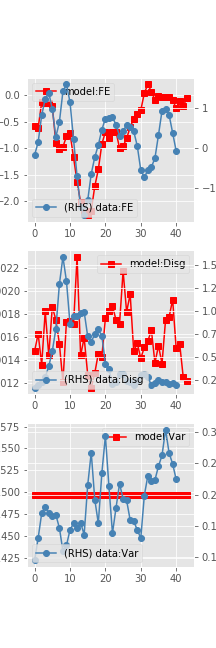
\includegraphics[width=\textwidth, height = 0.8\textheight]{figuresDraft/spf_ni_est_joint_diag0.png}
		\end{subfigure}
		\hfill
		\begin{subfigure}[b]{0.2\textwidth}
			\caption{Disg}
			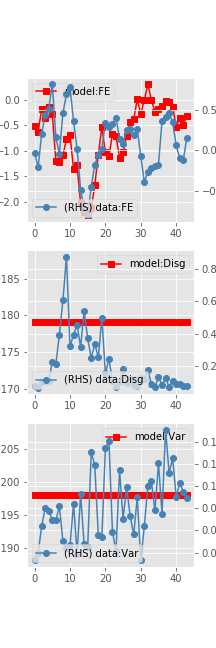
\includegraphics[width=\textwidth, height = 0.8\textheight]{figuresDraft/spf_ni_est_joint_diag1.png}
		\end{subfigure}
		\hfill
		\begin{subfigure}[b]{0.2\textwidth}
			\caption{FE/Disg}
			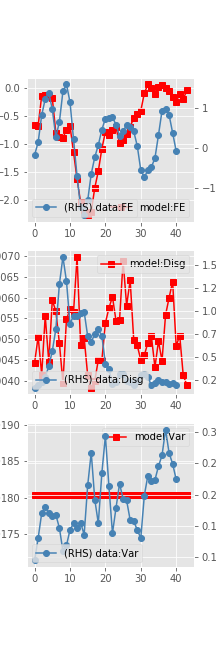
\includegraphics[width=\textwidth, height = 0.8\textheight]{figuresDraft/spf_ni_est_joint_diag2.png}
		\end{subfigure}
	\end{figure}
\end{frame}


\begin{frame}{Households and NIAR}
	\begin{figure}[ht]
		\label{NI_diag_SCE}
		\begin{subfigure}[b]{0.2\textwidth}
			\centering
			\caption{FE}
			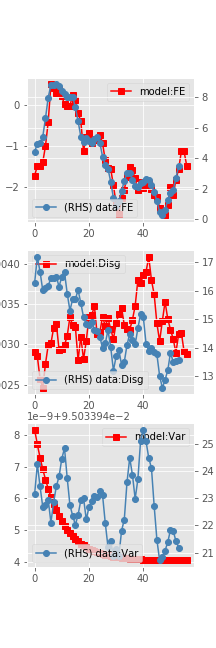
\includegraphics[width=\textwidth, height = 0.8\textheight]{figuresDraft/sce_ni_est_diag0.png}
		\end{subfigure}
		\hfill
		\begin{subfigure}[b]{0.2\textwidth}
			\caption{FE/Disg}
			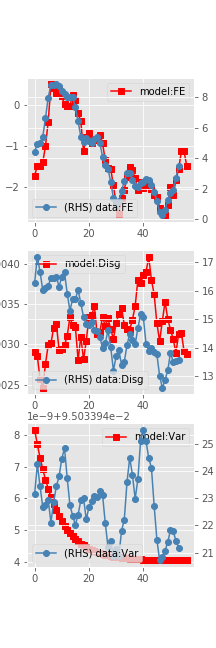
\includegraphics[width=\textwidth, height = 0.8\textheight]{figuresDraft/sce_ni_est_diag1.png}
		\end{subfigure}
		\hfill
		\begin{subfigure}[b]{0.2\textwidth}
			\caption{FE/Disg/Var}
			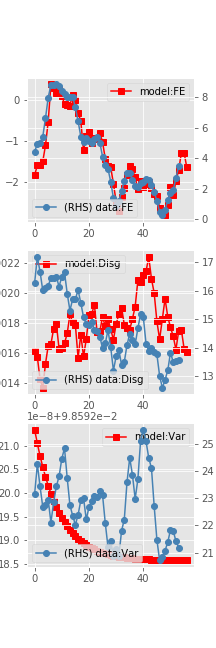
\includegraphics[width=\textwidth, height = 0.8\textheight]{figuresDraft/sce_ni_est_diag2.png}
		\end{subfigure}
		\end{figure}
\end{frame}


\begin{frame}{Households and NIAR: joint estimates}
	\begin{figure}[ht]
		\label{NI_diag_SCE_joint}
		\begin{subfigure}[b]{0.2\textwidth}
			\centering
			\caption{FE}
			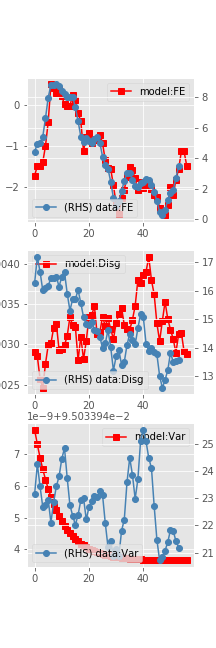
\includegraphics[width=\textwidth, height = 0.8\textheight]{figuresDraft/sce_ni_est_joint_diag0.png}
		\end{subfigure}
		\hfill
		\begin{subfigure}[b]{0.2\textwidth}
			\caption{FE/Disg}
			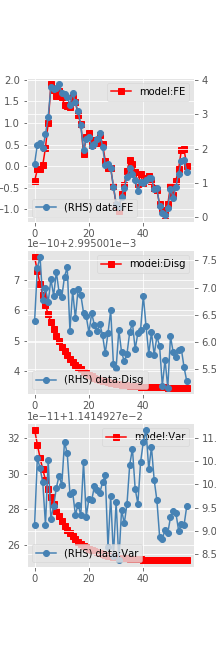
\includegraphics[width=\textwidth, height = 0.8\textheight]{figuresDraft/sce_ni_est_joint_diag1.png}
		\end{subfigure}
		\hfill
		\begin{subfigure}[b]{0.2\textwidth}
			\caption{FE/Disg/Var}
			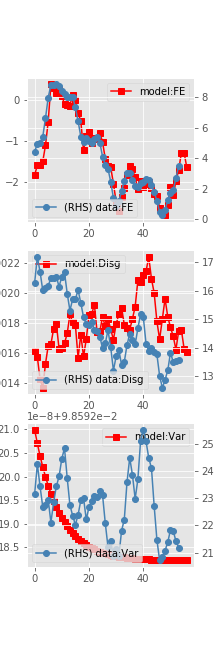
\includegraphics[width=\textwidth, height = 0.8\textheight]{figuresDraft/sce_ni_est_joint_diag2.png}
		\end{subfigure}
	\end{figure}
\end{frame}


\begin{comment}
%%%%%%%%%%%%%%%%%%%
\subsubsection{Hybird of NI and SE}


\begin{frame}{SENIAR parameters}
	\begin{table}
		\centering
		\caption{SMM Estimates of SENI}
		\label{SMM_Est_SENI_Table}
		\adjustbox{max height=0.5\textheight, max width=\textwidth}{ 
		\begin{tabular}{lllllllllllll}
			\hline 
			0  & 1     & 2     & 3    & 4       & 5       & 6   & SENI: $\lambda$ & SENI: $\sigma_{pb,SPF}$ & SENI: $\sigma_{pr,SPF}$ & SENI: $\lambda$ & SENI: $\sigma_{pb,SCE}$ & SENI: $\sigma_{pr,SCE}$ \\
			\hline 
			FE & FEVar & FEATV &      &         &         &     & 0.64            & 0.16                    & 0                       & 0.19            & 0.2                     & 0.21                    \\
			FE & FEVar & FEATV & Disg & DisgVar & DisgATV &     & 0.62            & 4.77                    & 0.17                    & 0.25            & 0.1                     & 0.35                    \\
			FE & FEVar & FEATV & Disg & DisgVar & DisgATV & Var & 0.62            & 13.7                    & 0.17                   & NA              & NA                      & NA                     \\
			\hline 
		\end{tabular}
		}
	\end{table}	
	\begin{itemize}
		\item $\sigma_{pb}$: noisiness of public signals in NI
		\item $\sigma_{pr}$: noisiness of private signals in NI
	\end{itemize}
\end{frame}


\begin{frame}{Professionals and SENIAR}
	\begin{figure}[ht]
		\label{SENI_diag_SPF}
		\begin{subfigure}[b]{0.2\textwidth}
			\centering
			\caption{FE}
			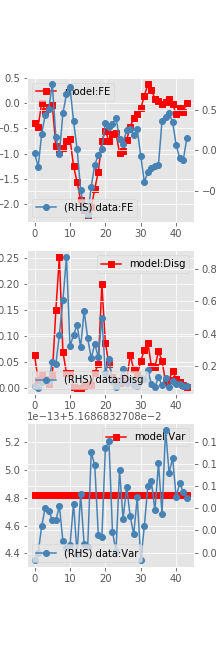
\includegraphics[width=\textwidth, height = 0.8\textheight]{figuresDraft/spf_seni_est_diag0.png}
		\end{subfigure}
		\hfill
		\begin{subfigure}[b]{0.2\textwidth}
			\caption{FE/Disg}
			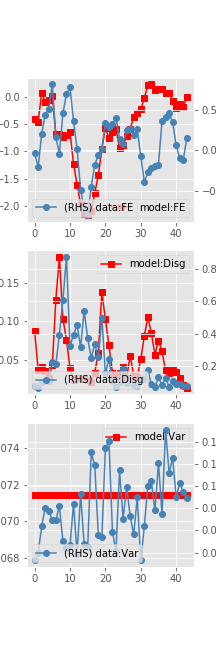
\includegraphics[width=\textwidth, height = 0.8\textheight]{figuresDraft/spf_seni_est_diag1.png}
		\end{subfigure}
		\hfill
		\begin{subfigure}[b]{0.2\textwidth}
			\caption{FE/Disg/Var}
			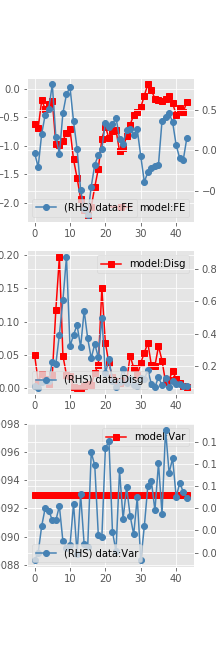
\includegraphics[width=\textwidth, height = 0.8\textheight]{figuresDraft/spf_seni_est_diag2.png}
		\end{subfigure}
	\end{figure}
\end{frame}



\begin{frame}{Households and SENIAR}
	\begin{figure}[ht]
		\label{SENI_diag_SCE}
		\begin{subfigure}[b]{0.2\textwidth}
			\centering
			\caption{FE}
			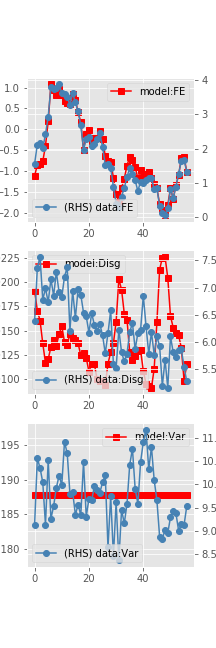
\includegraphics[width=\textwidth, height = 0.8\textheight]{figuresDraft/sce_seni_est_diag0.png}
		\end{subfigure}
		\hfill
		\begin{subfigure}[b]{0.2\textwidth}
			\caption{FE/Disg}
			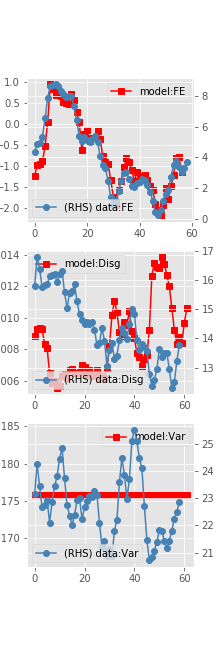
\includegraphics[width=\textwidth, height = 0.8\textheight]{figuresDraft/sce_seni_est_diag1.png}
		\end{subfigure}
		\hfill
		\begin{subfigure}[b]{0.2\textwidth}
			\caption{FE/Disg}
			\includegraphics[width=\textwidth, height = 0.8\textheight]{figuresDraft/sce_seni_est_diag2.png}
		\end{subfigure}
	\end{figure}
\end{frame}


\end{comment}


\subsection{Stocastic volatility}


\subsubsection{SE}



\begin{frame}{SESV parameters}
	\begin{table}
		\centering
		\caption{SMM Estimates of Parameters of SESV}
		\label{SMM_Est_SE_SV_Table}
		\adjustbox{max height=0.5\textheight, max width=\textwidth}{ 
\begin{tabular}{llllllllll}
	\hline 
	0       & 1       & 2       & 3   & SE: $\hat\lambda_{SPF}$(Q) & SE: $\hat\lambda_{SPF}$(Q) & SE: $\gamma$ & SE: $\hat\lambda_{SCE}$(M) & SE: $\hat\lambda_{SCE}$(M) & SE: $\gamma$ \\
	\hline 
	DisgATV & Var     &         &     & 0.3                        & 0.46                       & 2.52         & 0.09                       & 0.09                       & 0.7          \\
	FEATV   & DisgVar & DisgATV &     & 0.3                        & 0.46                       & 2.53         & 0.07                       & 0.07                       & 0.26         \\
	FEATV   & DisgVar & DisgATV & Var & 0.3                        & 0.46                       & 1.26         & 0.07                       & 0.07                       & 0.26        \\
	\hline 
\end{tabular}
		}
		\begin{itemize}
			\item $\lambda$: update rate in SE
				\item $\gamma$: size of the innovation to volatility	
		\end{itemize}
	\end{table}	
\end{frame}

\begin{frame}{Professionals and SESV}
	\begin{figure}[ht]
		\label{SESV_diag_SPF}
		\begin{subfigure}[b]{0.2\textwidth}
			\centering
			\caption{FE}
			\includegraphics[width=\textwidth, height = 0.8\textheight]{figuresDraft/spf_se_est_sv_diag0.png}
		\end{subfigure}
		\hfill
		\begin{subfigure}[b]{0.2\textwidth}
			\caption{Disg}
			\includegraphics[width=\textwidth, height = 0.8\textheight]{figuresDraft/spf_se_est_sv_diag1.png}
		\end{subfigure}
		\hfill
		\begin{subfigure}[b]{0.2\textwidth}
			\caption{FE/Disg}
			\includegraphics[width=\textwidth, height = 0.8\textheight]{figuresDraft/spf_se_est_sv_diag2.png}
		\end{subfigure}
	\end{figure}
\end{frame}



\begin{frame}{Professionals and SESV: joint estimates}
	\begin{figure}[ht]
		\label{SESV_diag_joint_SPF}
		\begin{subfigure}[b]{0.2\textwidth}
			\centering
			\caption{FE}
			\includegraphics[width=\textwidth, height = 0.8\textheight]{figuresDraft/spf_se_est_sv_joint_diag0.png}
		\end{subfigure}
		\hfill
		\begin{subfigure}[b]{0.2\textwidth}
			\caption{Disg}
			\includegraphics[width=\textwidth, height = 0.8\textheight]{figuresDraft/spf_se_est_sv_joint_diag1.png}
		\end{subfigure}
		\hfill
	\begin{subfigure}[b]{0.2\textwidth}
		\caption{Disg}
		\includegraphics[width=\textwidth, height = 0.8\textheight]{figuresDraft/spf_se_est_sv_joint_diag2.png}
	\end{subfigure}
	\end{figure}
\end{frame}


\begin{frame}{Households and SESV}
	\begin{figure}[ht]
		\label{SESV_diag_SCE}
		\begin{subfigure}[b]{0.2\textwidth}
			\centering
			\caption{Disg/Var}
			\includegraphics[width=\textwidth, height = 0.8\textheight]{figuresDraft/sce_se_est_sv_diag0.png}
		\end{subfigure}
		\hfill
		\begin{subfigure}[b]{0.2\textwidth}
			\caption{FE/Disg}
			\includegraphics[width=\textwidth, height = 0.8\textheight]{figuresDraft/sce_se_est_sv_diag1.png}
		\end{subfigure}
	\hfill	\begin{subfigure}[b]{0.2\textwidth}
		\caption{FE/Disg/Var}
		\includegraphics[width=\textwidth, height = 0.8\textheight]{figuresDraft/sce_se_est_sv_diag2.png}
	\end{subfigure}
	\end{figure}
\end{frame}


\begin{frame}{Households and SESV: joint estimates}
	\begin{figure}[ht]
		\label{SESV_diag_joint_SCE}
		\begin{subfigure}[b]{0.2\textwidth}
			\centering
			\caption{Disg/Var}
			\includegraphics[width=\textwidth, height = 0.8\textheight]{figuresDraft/sce_se_est_sv_joint_diag0.png}
		\end{subfigure}
		\hfill
		\begin{subfigure}[b]{0.2\textwidth}
			\caption{FE/Disg}
			\includegraphics[width=\textwidth, height = 0.8\textheight]{figuresDraft/sce_se_est_sv_joint_diag1.png}
		\end{subfigure}
		\hfill
		\begin{subfigure}[b]{0.2\textwidth}
			\caption{FE/Disg/Var}
			\includegraphics[width=\textwidth, height = 0.8\textheight]{figuresDraft/sce_se_est_sv_joint_diag2.png}
		\end{subfigure}
	\end{figure}
\end{frame}

%%%%%%%%%%%%%%%%%%%%


\subsubsection{DE}



\begin{frame}{DESV parameters}
	\begin{table}
		\centering
		\caption{SMM Estimates of Parameters of DESV}
		\label{SMM_Est_DE_SV_Table}
		\adjustbox{max height=0.5\textheight, max width=\textwidth}{ 
			\begin{tabular}{lllllllllllllll}
				\hline 
				0     & 1     & 2       & 3       & 4   & DE: $\theta$ & $\sigma_\theta$ & DE: $\theta$ & $\sigma_\theta$ & $\gamma$ & DE: $\theta$ & $\sigma_\theta$ & DE: $\theta$ & $\sigma_\theta$ & $\gamma$ \\
				\hline 
				FE    & FEVar & FEATV   &         &     & -0.44        & 0.36            & -0.43        & 1.03            & 0.13     & 7.81         & 4.39            & 7.81         & 2.99            & 0.7      \\
				FEVar & FEATV & DisgVar & DisgATV &     & -0.44        & 0.27            & -0.44        & 0.27           & 0.3      & 7.64         & 6.46            & 7.64         & 6.46            & 0.7      \\
				FEVar & FEATV & DisgVar & DisgATV & Var & -0.43        & 0.26            & -0.43        & 0.26            & 0.14     & 1.03         & 0               & 1.03         & 0               & 0.2     \\
				\hline 
			\end{tabular}
		}
		\begin{itemize}
			
			\item $\theta$: representativeness parameter
			\item $\sigma_\theta$: dispersion of representativeness across population
			\item $\gamma$: size of the innovation to volatility	
		\end{itemize}
	\end{table}	
\end{frame}


\begin{frame}{Professionals and DESV}
	\begin{figure}[ht]
		\label{DESV_diag_SPF}
		\begin{subfigure}[b]{0.2\textwidth}
			\centering
			\caption{FE}
			\includegraphics[width=\textwidth, height = 0.8\textheight]{figuresDraft/spf_de_est_sv_diag0.png}
		\end{subfigure}
		\hfill
		\begin{subfigure}[b]{0.2\textwidth}
			\caption{FE/Disg}
			\includegraphics[width=\textwidth, height = 0.8\textheight]{figuresDraft/spf_de_est_sv_diag1.png}
		\end{subfigure}
		\hfill
		\begin{subfigure}[b]{0.2\textwidth}
			\caption{FE/Disg/Var}
			\includegraphics[width=\textwidth, height = 0.8\textheight]{figuresDraft/spf_de_est_sv_diag2.png}
		\end{subfigure}
	\end{figure}
\end{frame}


\begin{frame}{Professionals and DESV: joint estimates}
	\begin{figure}[ht]
		\label{DESV_diag_joint_SPF}
		\begin{subfigure}[b]{0.2\textwidth}
			\centering
			\caption{FE}
			\includegraphics[width=\textwidth, height = 0.8\textheight]{figuresDraft/spf_de_est_sv_joint_diag0.png}
		\end{subfigure}
		\hfill
		\begin{subfigure}[b]{0.2\textwidth}
			\caption{FE/Disg}
			\includegraphics[width=\textwidth, height = 0.8\textheight]{figuresDraft/spf_de_est_sv_joint_diag1.png}
		\end{subfigure}
		\hfill
		\begin{subfigure}[b]{0.2\textwidth}
			\caption{FE/Disg/Var}
			\includegraphics[width=\textwidth, height = 0.8\textheight]{figuresDraft/spf_de_est_sv_joint_diag2.png}
		\end{subfigure}
	\end{figure}
\end{frame}

%%%%%%%%%%%


\begin{frame}{Households and DESV}
	\begin{figure}[ht]
		\label{DESV_diag_SCE}
		\begin{subfigure}[b]{0.2\textwidth}
			\centering
			\caption{FE}
			\includegraphics[width=\textwidth, height = 0.8\textheight]{figuresDraft/sce_de_est_sv_diag0.png}
		\end{subfigure}
		\hfill
		\begin{subfigure}[b]{0.2\textwidth}
			\caption{FE/Disg}
			\includegraphics[width=\textwidth, height = 0.8\textheight]{figuresDraft/sce_de_est_sv_diag1.png}
		\end{subfigure}
		\hfill
		\begin{subfigure}[b]{0.2\textwidth}
			\caption{FE/Disg}
			\includegraphics[width=\textwidth, height = 0.8\textheight]{figuresDraft/sce_de_est_sv_diag2.png}
		\end{subfigure}
	\end{figure}
\end{frame}


\begin{frame}{Households and DESV: joint estimates}
	\begin{figure}[ht]
		\label{DESV_diag_joint_SCE}
		\begin{subfigure}[b]{0.2\textwidth}
			\centering
			\caption{FE}
			\includegraphics[width=\textwidth, height = 0.8\textheight]{figuresDraft/sce_de_est_sv_joint_diag0.png}
		\end{subfigure}
		\hfill
		\begin{subfigure}[b]{0.2\textwidth}
			\caption{FE/Disg}
			\includegraphics[width=\textwidth, height = 0.8\textheight]{figuresDraft/sce_de_est_sv_joint_diag1.png}
		\end{subfigure}
		\hfill
		\begin{subfigure}[b]{0.2\textwidth}
			\caption{FE/Disg/Var}
			\includegraphics[width=\textwidth, height = 0.8\textheight]{figuresDraft/sce_de_est_sv_joint_diag2.png}
		\end{subfigure}
	\end{figure}
\end{frame}


%%%%%%%%%%%%%%%%%%%%%%%%%


\subsubsection{NI}

\begin{frame}{NISV parameters}
	\begin{table}
		\centering
		\caption{SMM Estimates of Parameters of NISV}
		\label{SMM_Est_NI_SV_Table}
		\adjustbox{max height=0.5\textheight, max width=\textwidth}{ 
			\begin{tabular}{llllllllllll}
				\hline 
				0       & 1       & 2       & 3       & 4   & NI: $\hat\sigma_{pb,SPF}$ & $\hat\sigma_{pr,SPF}$ & NI: $\hat\sigma_{pb,SPF}$ & $\hat\sigma_{pr,SPF}$ & $\gamma$ & NI: $\hat\sigma_{pb,SCE}$ & $\hat\sigma_{pr,SCE}$ \\
				\hline 
				FEVar   & FEATV   & Var     &         &     & 2.35                      & 2                     & 2.04                      & 23.01                 & 2.53     & 2.00014E+14               & 3.63                  \\
				FEVar   & FEATV   & DisgVar & DisgATV & Var & 3.33                      & 1.71                  & 2.04                      & 22.96                 & 2.53     & 1.09884E+13               & 3.63            \\
				\hline      
			\end{tabular}
		}
		\begin{itemize}
			\item $\sigma_{pb}$: noisiness of public signals in NI
			\item $\sigma_{pr}$: noisiness of private signals in NI
			\item $\gamma$: size of the innovation to volatility	
		\end{itemize}
	\end{table}	
\end{frame}


\begin{frame}{Professionals and NISV}
	\begin{figure}[ht]
		\label{NISV_diag_SPF}
		\begin{subfigure}[b]{0.2\textwidth}
			\centering
			\caption{FE/Var}
			\includegraphics[width=\textwidth, height = 0.8\textheight]{figuresDraft/spf_ni_est_sv_diag0.png}
		\end{subfigure}
		\hfill
		\begin{subfigure}[b]{0.2\textwidth}
			\caption{FE/Disg/Var}
			\includegraphics[width=\textwidth, height = 0.8\textheight]{figuresDraft/spf_ni_est_sv_diag3.png}
		\end{subfigure}
	\end{figure}
\end{frame}


\begin{frame}{Professionals and NISV: joint estimates}
	\begin{figure}[ht]
		\label{NISV_diag_joint_SPF}
		\begin{subfigure}[b]{0.2\textwidth}
			\centering
			\caption{FE/Var}
			\includegraphics[width=\textwidth, height = 0.8\textheight]{figuresDraft/spf_ni_est_sv_joint_diag0.png}
		\end{subfigure}
		\hfill
		\begin{subfigure}[b]{0.2\textwidth}
			\caption{FE/Disg/Var}
			\includegraphics[width=\textwidth, height = 0.8\textheight]{figuresDraft/spf_ni_est_sv_joint_diag3.png}
		\end{subfigure}
	\end{figure}
\end{frame}



\begin{frame}{Households and NISV}
	\begin{figure}[ht]
		\label{NISV_diag_SCE}
		\begin{subfigure}[b]{0.2\textwidth}
			\centering
			\caption{FE/Var}
			\includegraphics[width=\textwidth, height = 0.8\textheight]{figuresDraft/sce_ni_est_sv_diag0.png}
		\end{subfigure}
		\hfill
		\begin{subfigure}[b]{0.2\textwidth}
			\caption{FE/Disg/Var}
			\includegraphics[width=\textwidth, height = 0.8\textheight]{figuresDraft/sce_ni_est_sv_diag3.png}
		\end{subfigure}
	\end{figure}
\end{frame}


\begin{frame}{Households and NISV: joint estimates}
	\begin{figure}[ht]
		\label{NISV_diag_joint_SCE}
		\begin{subfigure}[b]{0.2\textwidth}
			\centering
			\caption{FE/Var}
			\includegraphics[width=\textwidth, height = 0.8\textheight]{figuresDraft/sce_ni_est_sv_joint_diag0.png}
		\end{subfigure}
		\hfill
		\begin{subfigure}[b]{0.2\textwidth}
			\caption{FE/Disg/Var}
			\includegraphics[width=\textwidth, height = 0.8\textheight]{figuresDraft/sce_ni_est_sv_joint_diag3.png}
		\end{subfigure}
	\end{figure}
\end{frame}


\begin{frame}{Taking stock}
	\begin{table}[]
		\caption{A scoring card of different theory} 
		\begin{tabular}{llll}
				\hline 
			Criteria                                    & SE     & NI  & DE     \\
				\hline 
			Sensitive to moments used for estimation?   & No     & No  & No     \\
			Sensitive to the assumed inflation process? & No     & Yes & No     \\
			Sensitive to a two-step or joint estimate?  & No     & Yes & No     \\
			Sensitive to the type of agents?            & Yes    & Yes & Yes    \\
			Matching with FE                            & Yes    & Yes & Yes    \\
			Matching with disagreement                  & Yes    & No  & Unsure \\
			Matching with uncertainty                   & Unsure & No  & No    \\
			\hline 
		\end{tabular}
	\end{table}
	
\end{frame}
%%%%%%%%%%%%%%%%%%%%%%%%%%%%%%%%%



\section{Conclusion}

\begin{frame}{Conclusion}
	\begin{itemize}
		\item Sticky expectation (SE) augmented with stochastic volatility of inflation process matches data of inflation and expectations better than other theories for both professionals and households.
		\item Within each model,  households are more inconsistent  compared to professionals
		\item Incorporating higher moments, i.e. uncertainty,  helps ``discipline'' theories on expectation formation
		\item  Higher moments from surveys also contain useful information about the inflation dynamics itself
	\end{itemize}	
\end{frame}


\bibliographystyle{apalike}
\bibliography{ExpSlides}


\end{document}
